% !TeX spellcheck = en_GB
% %%% ***************** CHAPTER INSTRUMENTS, RETRIEVAL, MEPS, DATA PROCESSING ***************** %%%
\chapter{Methods}\label{ch:Methods}
% \textcolor{red}{\textbf{The overleaf file from the Methodology is here:} \\ \url{https://www.overleaf.com/13946091vphmgxbbxpyg}} \\
This chapter describes the instruments, the optimal estimation retrieval and the regional forecast model used in the scope of this study, to determine the snow water content in the vertical. The determination of required parameters from the measuring instruments in relation to the optimal estimation retrieval will be explained. The purpose of this study is to compare the vertical observations from the Haukeliseter measurement site and the output from the operational forecast model at the Norwegian Meteorological Institute for the extreme weather event during Christmas 2016. 
The last section will give an insight on how the data was analysed to compare the different systems. 
%%%%%%%%%%%%%%%%%%%%%%%%%%%%%%%%%%%%%%%%%%%%%%%%%%%%%%%%%%%%%%%%%%%%%%%%%%
%%%%%%%%%%%%%%%%%%%%%%%%%%%%%%%%%%%%%%%%%%%%%%%%%%%%%%%%%%%%%%%%%%%%%%%%%%
% %%% ***************** CHAPTER Instruments ***************** %%%
% !TeX spellcheck = en_GB
\section{Instruments} \label{sec:DIM}


Many factors such as humidity and temperature contribute to snowflake geometry. The knowledge of snowflake habits, particle size distributions, and fall speed lead to a reduction of errors in optimal estimation retrievals. \\
This work is based on several datasets collected at the Haukeliseter measurement site, \ang{59.8}\,N, \ang{7.2}\,E. A composition of advanced ground-based observations and the CloudSat precipitation retrieval will help to get a better understanding of the vertical structure of the atmosphere. 
\\
%%%%%%%%%%%%%%%%%%%%%%%%%%%%%%%%%%%%%%%%%%%%%%%%%%%%%%%%%%%%%%%%%%%%%%%%%%
%%%%%%%%%%%%%%%%%%%%%%%%%%%%%%%%%%%%%%%%%%%%%%%%%%%%%%%%%%%%%%%%%%%%%%%%%%
%%%%%%%%% INTSTRUMENTS %%%%%%%%%%%%%%
%\section{Instruments}\label{sec:instruments}
A collaboration between the University of Utah, University of Wisconsin and Met-Norway made it possible to install three additional instruments at the measurement site during winter 2016/2017. A Multi-Angle Snowflake Camera (MASC) and a Precipitation Imaging Package (PiP) will be used to determine the snow habit, the snowfall particle size distribution, and near-surface fall speed. Additionally, a Micro Rain Radar (MRR) is established to obtain fall speed and particle reflectivity aloft. Together with temperature observations at the surface, is this a good basis to reduce the non-uniqueness of snow accumulation in optimal estimation snowfall retrieval, described in \Cref{sec:retrieval}. 
%%% image instrument setting @ Haukeli %%%%%%%%%%%%%%%%%%%%%%%%%%%%%%%%%%%%%
% !TeX spellcheck = en_GB

\begin{figure}
\centering
	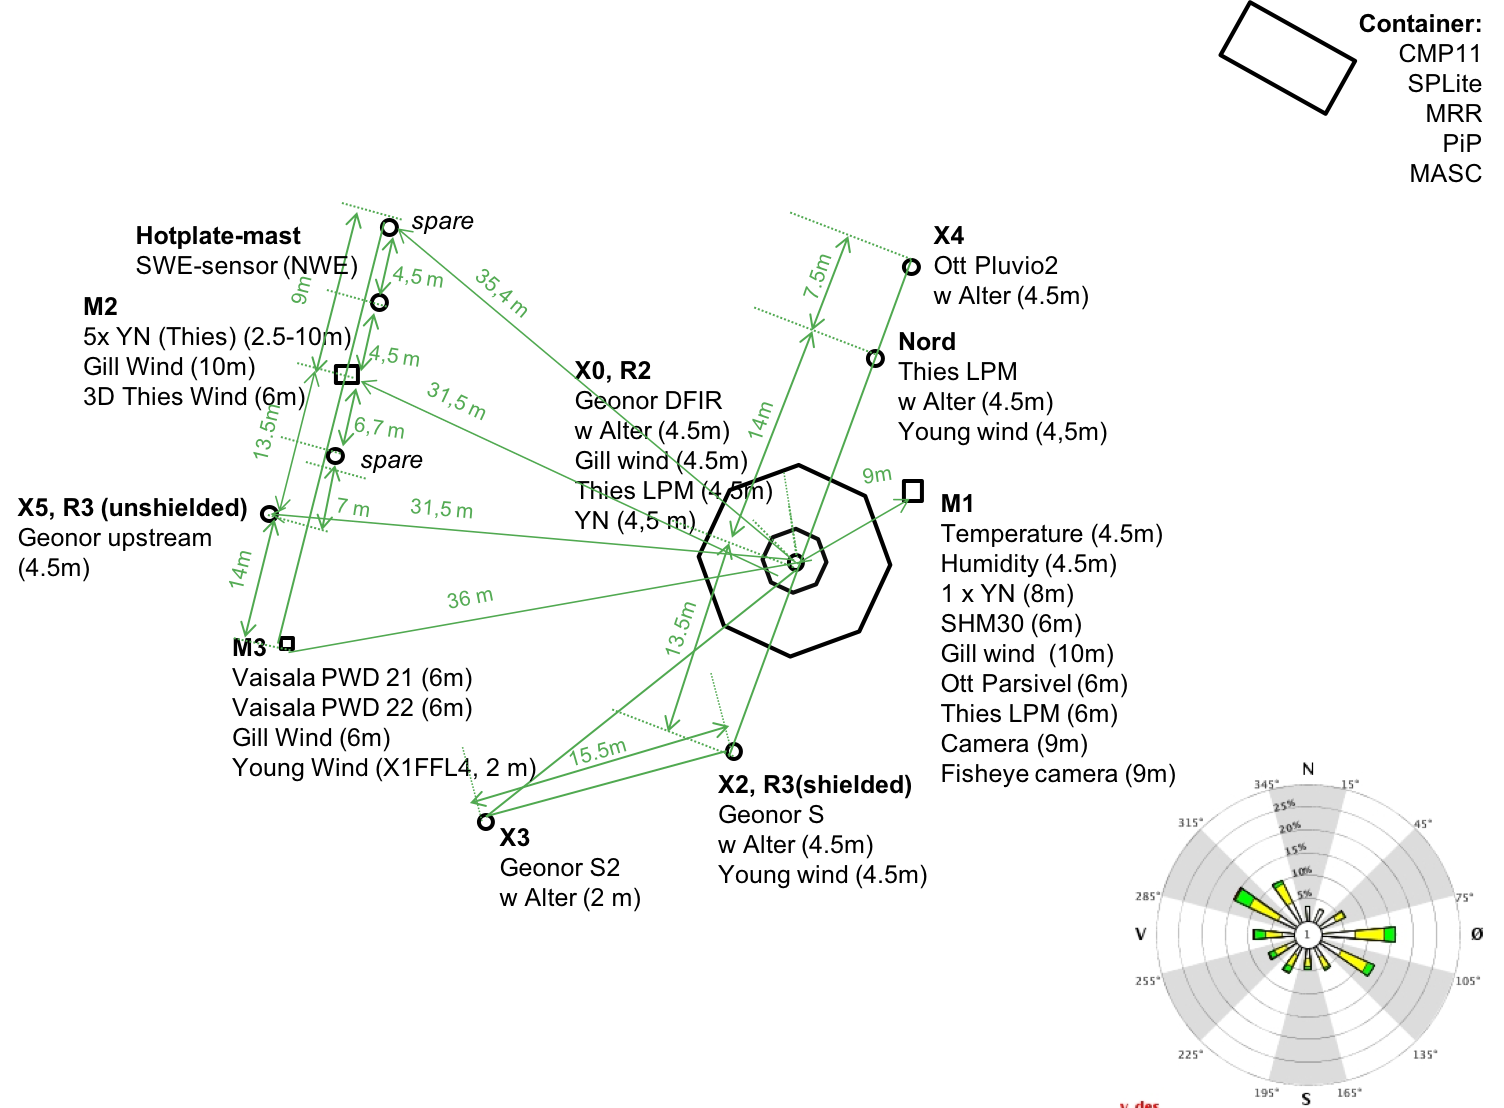
\includegraphics[width=\textwidth]{./fig_instruments/instrument_setting.png}
	%	\vspace{-10pt}
	\caption{Instruments at the Haukeliseter measurement site during winter 2016/2017 \citep[adapdet from][]{wolff_derivation_2015}. The windrose indicates the mean wind direction from either from west-north-west or east-south-east.}\label{fig:inst_setting}
\end{figure}

%%%%%%%%%%%%%%%%%%%%%%%%%%%%%%%%%%%%%%%%%%%%%%%%%%%%%%%%%%%%%%%%%%%%%%%%%%
\noindent
A sketch of the instrumentation setting is presented in \Cref{fig:inst_setting}. The octagonal indicates the double fence. The container is north-east from the double fence having the MRR, MASC and PiP mounted at the top. \textbf{M1} in \Cref{fig:inst_setting} is the \SI{10}{\metre} weather mast, providing the hourly \citet{eklima_norwegian_2016} temperature, pressure, and wind measurements. The mean wind direction from west-north-west and east-south-east are shown in the wind rose in \Cref{fig:inst_setting}.
%
%
%\pagebreak
%%%%%%%%%%%%%%%%%%%%%%%%%%%%%%%%%%%%%%%%%%%%%%%%%%%%%%%%%%%%%%%%%%%%%%%%%%
%%%%%%%%%%%%%%%%%%%%%%%%%%%%%%%%%%%%%%%%%%%%%%%%%%%%%%%%%%%%%%%%%%%%%%%%%%
%%%%%%%%% DOUBLE FENCE %%%%%%%%%%%%%%
\subsection{Double Fence}\label{sec:dofe}
%%% image double fence @ Haukeli %%%%%%%%%%%%%%%%%%%%%%%%%%%%%%%%%%%%%
% !TeX spellcheck = en_GB
% \begin{figure}[h!]
% 	\centering
% 		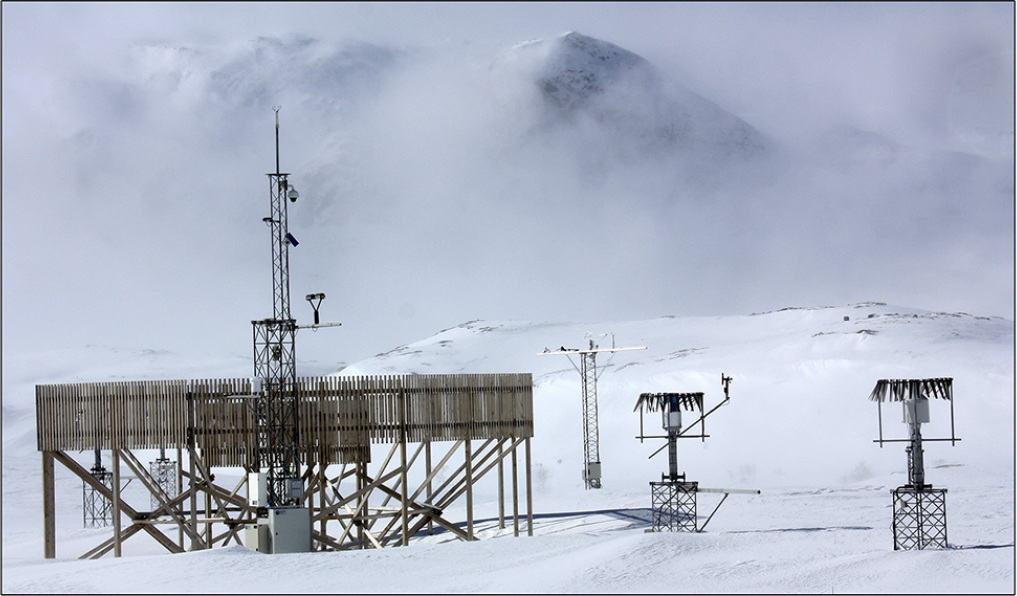
\includegraphics[width=0.55\textwidth]{./fig_instruments/Dofe.png}
% 	\caption{Picture, showing the double fence and unprotected precipitation gauges at the measurement site Haukeliseter. Picture taken from \cite{wolff_derivation_2015}.}\label{fig:Dofe}
% \end{figure}



\begin{wrapfigure}[28]{r}{0.44\textwidth}
	\vspace{-\normalbaselineskip}
	\centering
	\begin{subfigure}[b]{0.4\textwidth}
		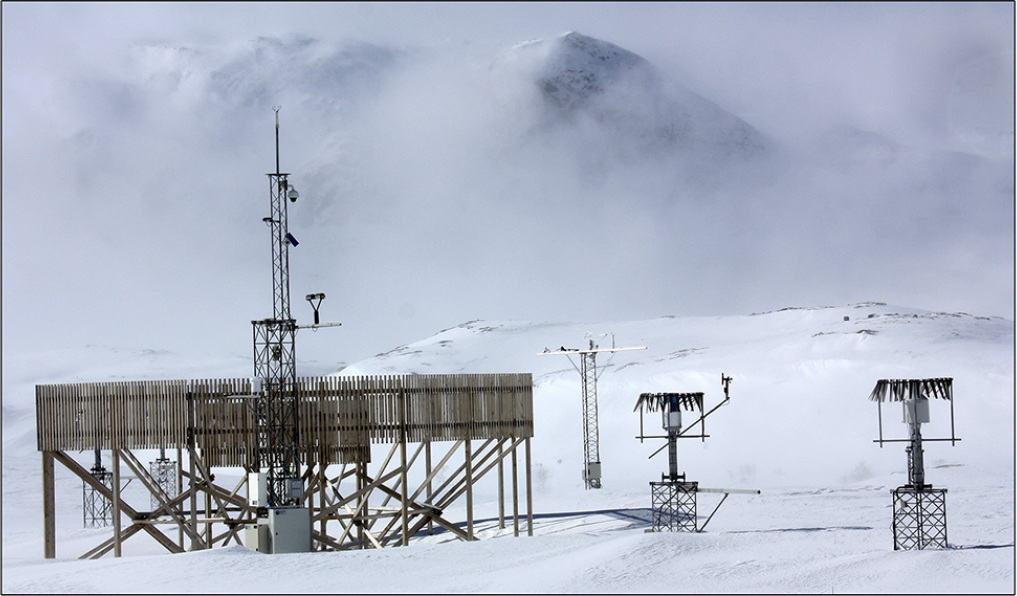
\includegraphics[width=\textwidth]{./fig_instruments/Dofe.png}
		\caption{}\label{fig:dofe_pic}
	\end{subfigure}	
	\begin{subfigure}[b]{0.4\textwidth}
		% 		\includegraphics[trim={0.8cm, 2.3cm, 2.4cm, 3cm},clip,width=1.1\textwidth]
		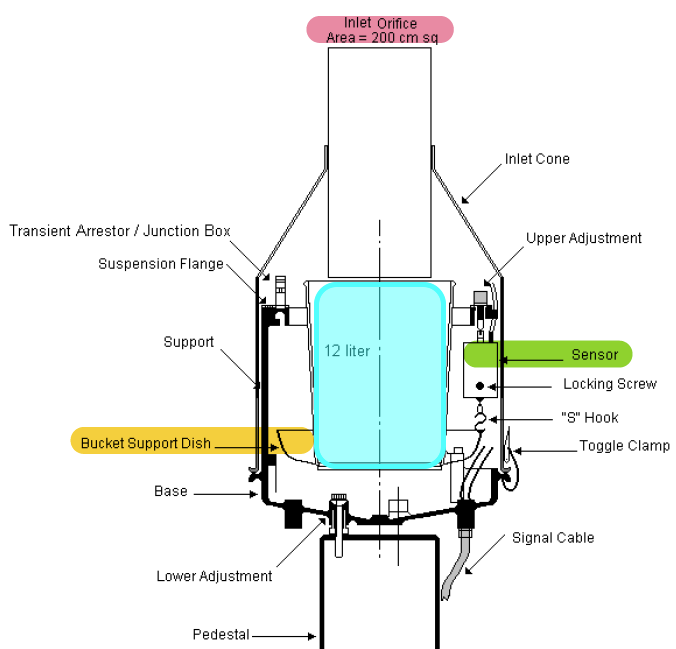
\includegraphics[width=1.1\textwidth]{./fig_instruments/Geonor_sketch2.png}
		\caption{}\label{fig:gauge_sketch}
	\end{subfigure}	
	\caption{(\protect\subref{fig:dofe_pic}) From left to right: Double fence gauge (\textbf{X0}) and unprotected precipitation gauges (\textbf{Nord, X4}) at Haukeliseter, from \cite{wolff_derivation_2015}. The prevailing easterly (westerly) wind from the lower, left corner in \protect\subref{fig:dofe_pic} (the opposite site). In front of the double fence gauge is the \SI{10}{\metre} weather mast (\textbf{M1}). (\protect\subref{fig:gauge_sketch}) Vertical cross section of Geonor T-200B3 precipitation gauge. pink: orifice; cyan: cylindric bucket with frost protection; yellow: bucket support dish; green: wire sensor \citep[adapted from][]{geonor_inc._t-200b_2015}.  }\label{fig:Dofe}
	%	\vspace{-\normalbaselineskip}
\end{wrapfigure}
%%%%%%%%%%%%%%%%%%%%%%%%%%%%%%%%%%%%%%%%%%%%%%%%%%%%%%%%%%%%%%%%%%%%%%%%%%
Since the winter season 2010/2011 Haukeliseter is equipped with several precipitation gauges. The wind shielded gauges are placed perpendicular to the main wind direction (E/W wind).
\\
In a study by \citet{wolff_derivation_2015} the wind-induced under-catch of solid precipitation is determined. Dependent on the kind of precipitation the wind plays different roles in the amount of accumulation. For temperatures below \SI{-2}{\celsius} the wind speed influences the falling snow. Where less precipitation can be observed at higher wind speeds or more precipitation can be measured if too much is blown into the gauge. The catch ratio between the standard Geonor precipitation gauge and the Double Fence - Geonor (\Cref{fig:dofe_pic}) shows, that only \SI{80}{\percent} of solid precipitation are observed at wind speeds of \SI{2}{\mPs} and only \SI{40}{\percent} at \SI{5}{\mPs}, \citet[Figure 5 in][]{wolff_derivation_2015}. 
\\
The precipitation gauge protected by an octagonal double fence (\Cref{fig:dofe_pic}) is more accurate than the single fence and will be used as the reference to all surface accumulation measurements. The double fence creates an artificial calm wind and maximize the catch of precipitation, \citep{wolff_new_2010, wolff_measurements_2013, wolff_derivation_2015}. The wind inside the double fence is measured to be not much higher than \SI{5}{\mPs} even if the winds outside exceed \SI{20}{\mPs} (occurred \SI{26}{\dec}). % so far it is unknown, if the catch efficiency stabilises for wind speeds beyond \SI{10}{\mPs} and may lead to wrong values
\\
This shows the need of a combination of ground-based observations together with an optimal estimation retrieval to verify the accuracy of MEPS. \citet{wolff_derivation_2015} introduced an adjustment function for the Geonor double fence, so that different precipitation under certain wind speeds are presented correctly and can be used as confidential data. 
For now, it is presumed that the average under catch inside a double fence is \SI{20}{\percent} for wind speeds between \SIlist{10;20}{\mPs} and \SI{10}{\percent} for wind speeds under \SI{9}{\mPs} \citep{wolff_wmo_2018}.
\\ \\
Inside the double fence is a precipitation-weighing gauge Geonor T-200B3 \citep[3-wire transducers, \SI{1000}{\mm},][]{geonor_inc._t-200b_2015} with an Alter wind screen to reduce wind turbulence around the gauge. At Haukeliseter is the orifice height of the Geonor \SI{4.5}{\metre} above the ground. This is due to an expected snow depth of \SIrange{2}{3}{\metre} during a winter season and to reduce the likelihood of measuring drifting snow \citep{wolff_measurements_2013,wolff_derivation_2015}. \\
A vertical cross section of the T-200B gauge is shown in \Cref{fig:gauge_sketch}. Precipitation particles fall through the \SI{200}{\square\cm} orifice protected with a heated collar, into a cylindric bucket filled with frost protection. The bucket is placed on top of a Bucket Support Dish \citep[\Cref{fig:gauge_sketch},][]{geonor_inc._t-200b_2015}. This dish is connected with three wire sensors having an eigenfrequency changing with the weight inside the bucket. A formula provided by \citet{geonor_inc._t-200b_2015} calculates the amount of precipitation from the frequency of each sensor. The three sensors provide a reduction of an error in connection with an unlevel installation. Met-Norway will average value of all three sensors and provide it as hourly data at \citeauthor{eklima_norwegian_2016}.
%%%%%%%%%%%%%%%%%%%%%%%%%%%%%%%%%%%%%%%%%%%%%%%%%%%%%%%%%%%%%%%%%%%%%%%%%%
%%%%%%%%%%%%%%%%%%%%%%%%%%%%%%%%%%%%%%%%%%%%%%%%%%%%%%%%%%%%%%%%%%%%%%%%%%
%%%%%%%%% MRR %%%%%%%%%%%%%%
\subsection{MRR - Micro Rain Radar}\label{sec:MRR}
%%% image MRR instrument %%%%%%%%%%%%%%%%%%%%%%%%%%%%%%%%%%%%%
% !TeX spellcheck = en_GB
% \begin{figure}[h!]
% 	\centering
% 		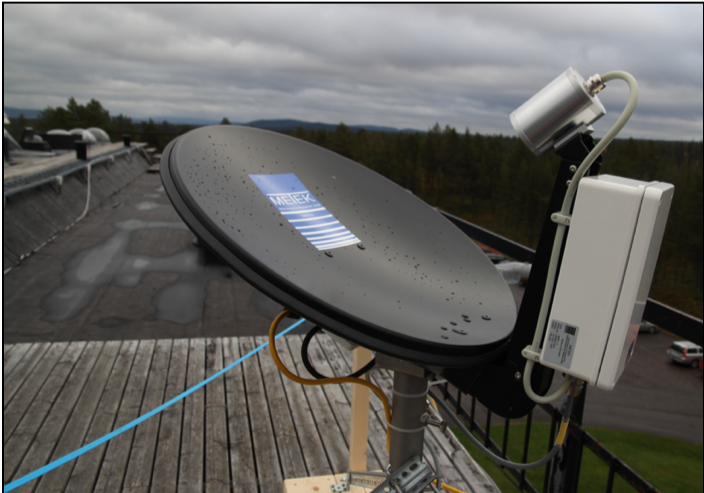
\includegraphics[width=0.55\textwidth]{./fig_instruments/MRR.png}
% 	\caption{MRR from METEK}\label{fig:MRR}
% \end{figure}

\begin{wrapfigure}[14]{r}{0.44\textwidth}
	\vspace{-\normalbaselineskip}
	\centering
	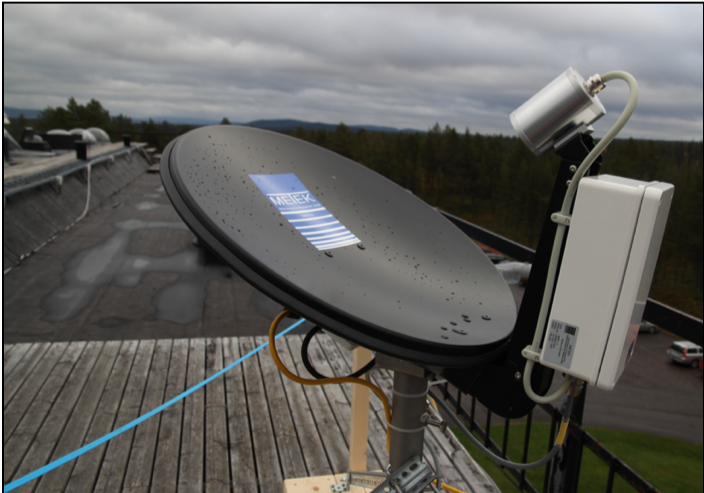
\includegraphics[width=0.4\textwidth]{./fig_instruments/MRR.png}
	%	\vspace{-10pt}
	\caption{Micro Rain Radar at the measurement site in Kiruna. Transceiver transmits Radar signal using the antenna (parabolic dish) and receives backscatter signal over the antenna. During winter 2016/2017 installed at Haukeliseter (\textbf{container}).}\label{fig:MRR}
	\vspace{-\normalbaselineskip}
\end{wrapfigure}
%%%%%%%%%%%%%%%%%%%%%%%%%%%%%%%%%%%%%%%%%%%%%%%%%%%%%%%%%%%%%%%%%%%%%%%%%%
Radars are very useful to observe the vertical of the atmosphere. The instrument is able to detect mesoscale features and makes it possible to see the vertical structure of storms \citep{markowski_mesoscale_2011}.\\
The principle of radar measurements is based on an electromagnetic wave, which is emitted from the radar transmitter and interacts with the hydrometeors along the beam. A fraction of the pulse energy is reflected back to the receiver of the radar. The quantity of scattering depends on the shape and structure of the reflected particle. 
Vertical profiles of reflectivity give information about the diameter of the target object.
\\
The Micro Rain Radar, in \Cref{fig:MRR}, measures profiles of Doppler spectra \citep{metek_micro_2010}. The Doppler spectrum tells about the movement of the particle. The vertical pointing Doppler radar measures the energy that is returned from each interval and thus enabling the detection of the Doppler spectrum \citep{lecuyer_aos_2017}. The MRR measures at a frequency of \SI{24}{\giga\Hz} and has a temporal and spatial resolution of \SI{60}{\second} and \SI{100}{\metre}, respectively. The radar height range is from \SI{100}{\metre} (because of ground clutter) to \SI{3.000}{\metre} \citep{metek_micro_2010}.
\\
MRR radar reflectivity ($Z$) is transformed from \SI{1}{\mm^6\per\metre^3} to \SI{}{\decibel\,Z}.
The transformations are done with the following relationship;
\begin{align}
	Ze & = 10 \log_{10} \left(\frac{Z}{\SI{1}{\mm^6\per\metre^3}}\right) \qquad [\SI{}{\decibel Z}]
	\label{eq:Ze}
\end{align}
A transformation to rainfall rates can be performed by the $Z$-$R$ (reflectivity - rainfall) relationship. 
The rainfall rate in each layer can be estimated by the use of typical fall speeds and the Marshall-Palmer particle size distribution for liquid particles \citep{rinehart_radar_2010}. 
\begin{align}
	Z & = 200 R^{\frac{8}{5}} \qquad [\SI{}{\mm^6\metre^{-3}} ] \nonumber \\ 
	R & = \left( \frac{ 10^{\frac{Ze}{10}} }{200} \right)^{\frac{8}{5}} \qquad [ \SI{}{\mm\per\hour} ]
	\label{eq:Z-R}
\end{align}
\\
\Cref{tab:ref_values} represents the Z-R relationship if the Marshall-Palmer assumption (\Cref{eq:Z-R}) is applied. Z-snowfall relationships are developed but are difficult to apply due to the variation of size and density of the particles \citep{lecuyer_aos_2017}. \\
After the transformation to \SI{}{\decibel Z} the reflectivity is averaged for every \SI{200}{\metre} layer thickness, where only values above \SI{300}{\metre} are taken. 
For instance, a reflectivity at \SI{400}{\metre} represents the mean value of reflectivity between \SIlist{300;500}{\metre}. 
%%% table REFLECTIVITY AND RAINRATE %%%%%%%%%%%%%%%%%%%%%%%%%%%%%%%%%%%%%
% % !TeX spellcheck = en_GB
\begin{table}[t]
	\begin{center}
		\caption{Typical reflectivity values, from \cite{doviak_doppler_1993}. The values are obtained from measurements, models and observations. The rainfall rate $R$ is calculated with \Cref{eq:Z-R}. }\label{tab:ref_values}
		\begin{tabular}{ll|c|c}
			\hline \hline
			\multicolumn{2}{l|}{} & \textbf{Ze} & \textbf{R} \\ 
			\multicolumn{2}{l|}{} & [\SI{}{\decibel Z}] & [\SI{}{\mm\per\hour}] \\ \hline \hline
			\multicolumn{2}{l|}{\textbf{Drizzle}} & \num{< 25} &  \num{1.3} \\ \hline
			\multicolumn{2}{l|}{\textbf{Rain}} & \numrange{25}{60} & \numrange{1.3}{205.0} \\ \hline
			\multicolumn{2}{l|}{\textbf{Snow}} &  \\ 
			& dry, low density 	& \num{< 35} & \num{5.6}\\ \hline
			& Crystal; dry, high density & \num{< 25} & \num{1.3}\\ \hline
			& wet, melting 		& \num{< 45} & \num{23.7} \\ \hline
			\multicolumn{2}{l|}{\textbf{Graupel}} & \\
			& dry 				& \numrange{40}{50} & \numrange{11.5}{48.6} \\ \hline
			& wet				& \numrange{40}{55} & \numrange{11.5}{99.9} \\ \hline
			\multicolumn{2}{l|}{\textbf{Hail}} & \\
			& small; \SI{< 2}{\cm}, wet & \numrange{50}{60} & \numrange{48.6}{205.0}\\
			& large; \SI{> 2}{\cm}, wet & \numrange{55}{70} & \numrange{99.9}{864.7}\\ \hline
			\multicolumn{2}{l|}{\textbf{Rain \& Hail}} & \numrange{50}{70} & \numrange{48.6}{864.7} \\ 
			\hline \hline
		\end{tabular}
	\end{center}
\end{table}
%%%%%%%%%%%%%%%%%%%%%%%%%%%%%%%%%%%%%%%%%%%%%%%%%%%%%%%%%%%%%%%%%%%%%%%%%%

\newpage
%%%%%%%%%%%%%%%%%%%%%%%%%%%%%%%%%%%%%%%%%%%%%%%%%%%%%%%%%%%%%%%%%%%%%%%%%%
%%%%%%%%%%%%%%%%%%%%%%%%%%%%%%%%%%%%%%%%%%%%%%%%%%%%%%%%%%%%%%%%%%%%%%%%%%
%%%%%%%%% PiP %%%%%%%%%%%%%%
\subsection{PiP - Precipitation Imaging Package}
%%% image PiP instrument %%%%%%%%%%%%%%%%%%%%%%%%%%%%%%%%%%%%%
% !TeX spellcheck = en_GB
% \begin{figure}[h!]
% 	\centering
% 		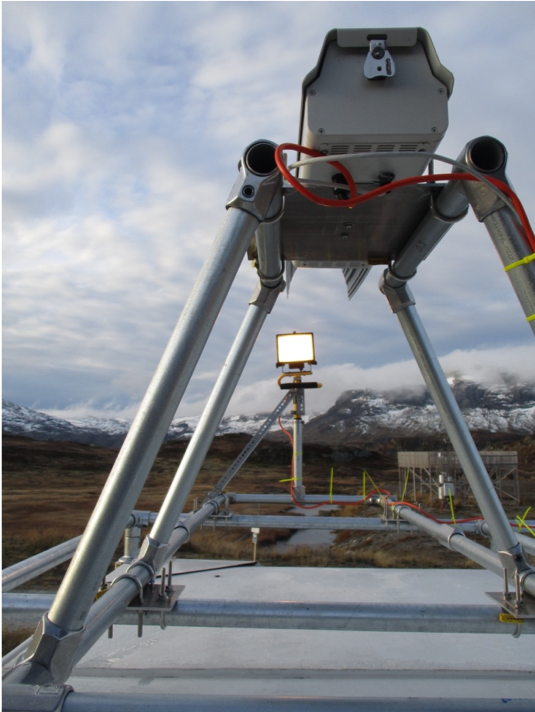
\includegraphics[width=0.35\textwidth]{./fig_instruments/PiP.png}
% 	\caption{PiP}\label{fig:PiP}
% \end{figure}

\begin{wrapfigure}[21]{r}{0.44\textwidth}
	\vspace{-\normalbaselineskip}
	\centering
	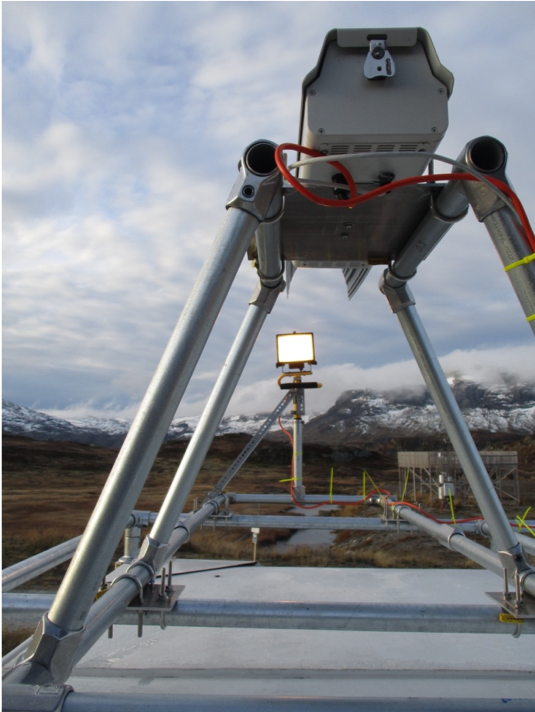
\includegraphics[trim={3.cm, 3.3cm, .5cm, 0cm},clip,width=0.4\textwidth]{./fig_instruments/PiP.png}
	%	\vspace{-10pt}
	\caption{Precipitation Imaging Package at Haukeliseter mounted at the \textbf{container} pointing towards the double fence gauge.}\label{fig:PiP}
	\vspace{-\normalbaselineskip}
\end{wrapfigure}
%%%%%%%%%%%%%%%%%%%%%%%%%%%%%%%%%%%%%%%%%%%%%%%%%%%%%%%%%%%%%%%%%%%%%%%%%%
The precipitation imaging package (PiP) is a modification of the Snowflake Video Imager presented by \citet{newman_presenting_2009}. The video distrometer is a construct of a halogen flood lamp and a video system (\Cref{fig:PiP}). The instrument determines the habit of snowflakes from images at a frequency of \SI{60}{\Hz}. Lamp and lens have a distance of approximately \SI{3}{\metre} which follows a field of view: \SI{32}{\mm} by \SI{24}{\mm}. 
\\
In front of the halogen lamp is a frosted window, so that the background light is uniform over all time. A falling particle appears as a 2-D shadow in the video image. 
Particle size distribution (PSD) and fall speed of precipitation can be determined from the black and white images of the system.
\citet{newman_presenting_2009} describes in detail the algorithm applied to the system to get information about the snow-particle habit. \\
Winds have almost no effect on the result of the video distrometer \citep{newman_presenting_2009}. To reduce eventual wind effects, was the distrometer oriented perpendicular to the mean wind.
\newpage
%%%%%%%%%%%%%%%%%%%%%%%%%%%%%%%%%%%%%%%%%%%%%%%%%%%%%%%%%%%%%%%%%%%%%%%%%%
%%%%%%%%%%%%%%%%%%%%%%%%%%%%%%%%%%%%%%%%%%%%%%%%%%%%%%%%%%%%%%%%%%%%%%%%%%
%%%%%%%%% MASC %%%%%%%%%%%%%%
\subsection{MASC - Multi-Angular Snowfall Camera}
%%% image MASC %%%%%%%%%%%%%%%%%%%%%%%%%%%%%%%%%%%%%
% !TeX spellcheck = en_GB
% \begin{figure}[h!]
% 	\centering
% 	\begin{subfigure}[b]{0.55\textwidth}
% 		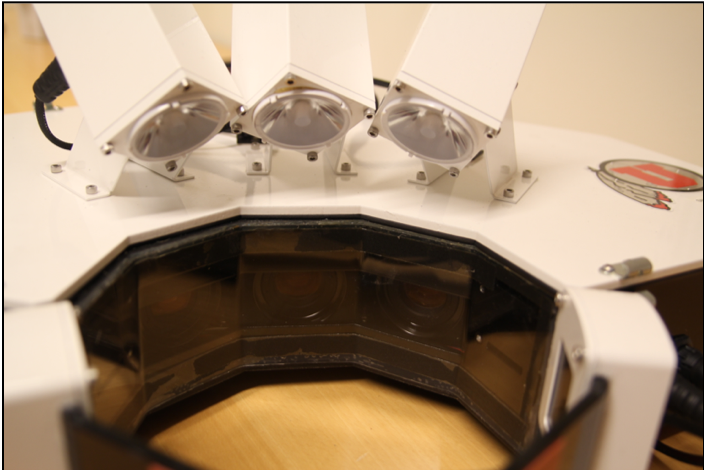
\includegraphics[width=\textwidth]{./fig_instruments/MASC.png}
% 	\end{subfigure}
% 	\begin{subfigure}[b]{0.55\textwidth}
% 		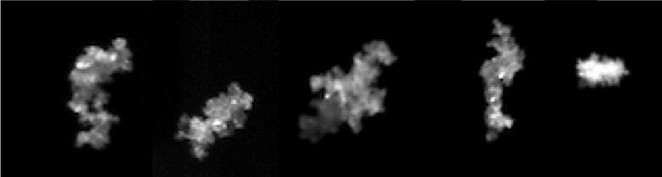
\includegraphics[width=\textwidth]{./fig_instruments/MASC_snowflakes.png}
% 	\end{subfigure}
% 	\caption{Instrument MASC, and images taken by the instrument. \textcolor{red}{lower panel taken from \cite{cooper_variational_2017} maybe we get one for Haukeli?}}\label{fig:MASC}
% \end{figure}

% \begin{wrapfigure}[17]{r}{0.44\textwidth}
\begin{wrapfigure}[15]{r}{0.44\textwidth}
	\vspace{-\normalbaselineskip}
	\centering
	\begin{subfigure}[b]{0.4\textwidth}
		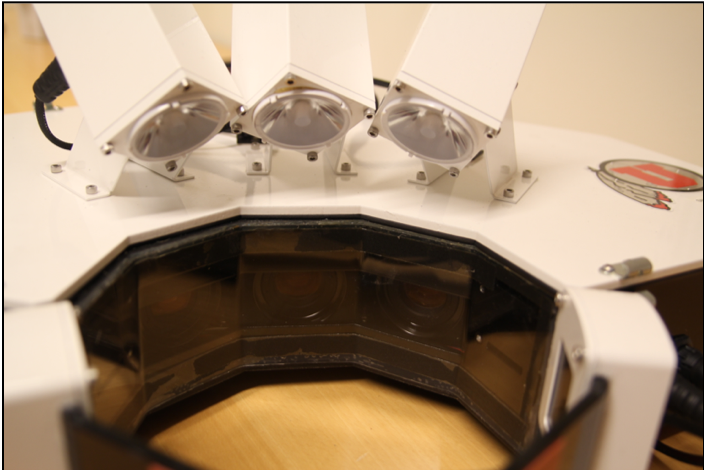
\includegraphics[trim={1.cm, 0cm, .8cm, 0cm},clip,width=\textwidth]{./fig_instruments/MASC.png}
	\end{subfigure}	
	\begin{subfigure}[b]{0.4\textwidth}
		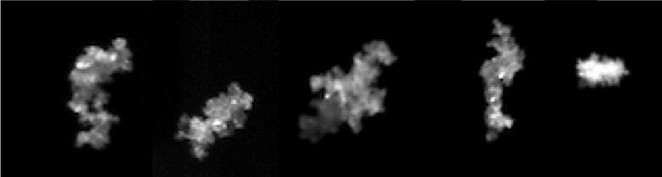
\includegraphics[width=\textwidth]{./fig_instruments/MASC_snowflakes.png}
	\end{subfigure}	
	\caption{Multi-Angular Snowfall Camera and images taken by the instrument during the Christmas storm 2016. Located on \textbf{container}.}\label{fig:MASC}
	%	\vspace{-\normalbaselineskip}
\end{wrapfigure}
%%%%%%%%%%%%%%%%%%%%%%%%%%%%%%%%%%%%%%%%%%%%%%%%%%%%%%%%%%%%%%%%%%%%%%%%%%
Instruments like the afore mentioned PiP has according to \citet{garrett_fall_2012} coarser resolution and the determination of particle size can have larger errors. Hence, a new instrument was developed. The Multi-Angular Snowfall Camera (MASC) takes high-resolution images of hydrometeors in free fall and measures the fall-speed simultaneously. \\
The MASC consists of three cameras, three flashes, and two near-infrared sensors, pointing at a ring centre (\Cref{fig:MASC}). A hydrometeor has to pass through the ring in a certain way to trigger the near-infrared sensors. At the same time the three cameras take a picture of the falling particle. Since the cameras take pictures from three different angles, the particles size, shape, and orientation can be specified from an algorithm applied to the image, described in \citet{garrett_fall_2012}. Furthermore, the form and heritage of the hydrometeor, such as collision-coalescence, riming, capture nucleation, or aggregation, can be determined. \\
The near-infrared sensor, that is used to trigger the cameras and the lights quantifies the fall-speed of the hydrometeors, by measuring the time the particle needs to pass the distance between the upper and lower trigger.    


%%%%%%%%%%%%%%%%%%%%%%%%%%%%%%%%%%%%%%%%%%%%%%%%%%%%%%%%%%%%%%%%%%%%%%%%%%
%%%%%%%%%%%%%%%%%%%%%%%%%%%%%%%%%%%%%%%%%%%%%%%%%%%%%%%%%%%%%%%%%%%%%%%%%%
% %%% ***************** CHAPTER RETRIEVAL ***************** %%%
% !TeX spellcheck = en_GB
\section{Optimal Estimation Retrieval Algorithm} %Section - 1.2
\label{sec:retrieval}
Since 2006, with the launch of CloudSats Cloud Profiling Radar (CPR) a global estimation of snowfall can be done. Several studies, such as \cite{kulie_utilizing_2009} have shown that estimated snowfall values depend heavily upon assumed snowflake microphysical properties.
%\textcolor{red}{Steve had some insertions but no comments.}
%depending on the retrieval assumption, snowfall estimation can give the same values for different a priori guess, e.g. snowflake microphysical properties. 
%Introducing information from snow microphysics will reduce the non-uniqueness in optimal estimation radar retrieval schemes. 
%This can be done by using the temperature at a lower level as a priori as the CloudSat retrieval does.  
%\\
\cite{wood_microphysical_2015} showed that a refinement of the CloudSat snowfall retrieval algorithm can be performed by using snowflake models. 
%\textcolor{red}{That was Steves comment which is exactly what I wrote? "
This study was based on data from the Canadian CloudSat-CALIPSO Validation Project \citep[C3VP,][]{hudak_canadian_2006}, where they concentrated on cold season clouds and precipitation.
%"} 
\\
\noindent In an attempt to reduce the non-uniquness of the problem, \cite{wood_microphysical_2015} used the a priori knowledge of snowfall microphysics and temperature (from ground-based observations) to refine the forward-model assumptions for the CloudSat snowfall retrieval scheme. 
%\textcolor{red}{Steve: "They also used a temperature to introduce a priori information on particle size into the retrieval scheme. " Me: They did? So by introducing a temp they estimate the particle size?}
Results from this scheme showed a good agreement with reported values observed at meteorological measurement sites. \\
Model estimates have proven, how useful the estimation retrieval can be to verify ground-based radar snowfall measurements \citep{norin_intercomparison_2015}.
Although the retrieval has obviously been improved the estimation algorithm, a priori guess can still lead to uncertainties in the retrievals of up to \SIrange{140}{200}{\percent} \citep{wood_estimation_2011}. 
\\
% \noindent The snowfall retrieval assumes an exponential particle size distribution (PSD)
% \begin{align}
% 	N(D) = N_{0} exp(-\lambda D).
% 	\label{eq:PSD}
% \end{align} 
% $\lambda$ represents here the PSD slope parameter and $N_{0}$ the number density. 
% %$D$ is the particle maximum dimension evaluated from the MASC. 
% \\
% The optimal estimation technique is based on Gaussian statistics. Minimizing the scalar cost function, $\Phi$ for the snowfall properties, $x$ by; 
% \begin{equation}
% \begin{split}
% \Phi(x,y,a) = &(y- F(x))^T \mathbf{S}_y^{-1} (\mathbf{y}-F(\mathbf{x})) \\
% &+(x-a)^T \mathbf{S}_{a}^{-1} (x-a)
% \end{split} \label{eq:scalar_cost_fct}
% \end{equation}
% where, $x$, vector of retrieved snowfall properties (slope parameter and number density); $y$, vector of observation (MRR reflectivity) ; $a$, vector of the a priori guess (temperature dependent); $F$, forward model; $\mathbf{S}_a$, a priori error covariance matrix; $\mathbf{S}_y$, measurement error covariance matrix.
% \\
\cite{cooper_variational_2017} developed a technique to combine MRR, MASC, and PiP information into a common retrieval framework. Specifically, estimates of snowflake microphysical properties from the MRR are used as the a priori term in the optimal-estimation retrieval scheme. The usage of either MASC/PiP or MRR fall-speed can show which a priori guess in the retrieval gives the more accurate retrieved snowfall rate at the ground. \\
The difference between the retrieval and the snow gauge observations was \SI{-18}{\percent} when applied to data from Barrow, Alaska.\\
\cite{cooper_variational_2017} also showed that the retrieval is sensitive to habit and fall speed. The installation of a MRR, MASC, and PIP should help to adjust the particle models for graupels and rimed particles which are often observed at Haukeliseter. 

\subsection{Presence of snow}\label{sec:pre_snow}
%\item surface temperature \SI{< 2}{\celsius}
%\item follows \Cref{fig:MRR_sfcT}
% %%% image surface temperature and MRR %%%%%%%%%%%%%%%%%%%%%%%%%%%%%%%%%%%%%
% !TeX spellcheck = en_GB
\begin{figure}[t!]
	\centering
	%    \begin{subfigure}[b]{\textwidth}
	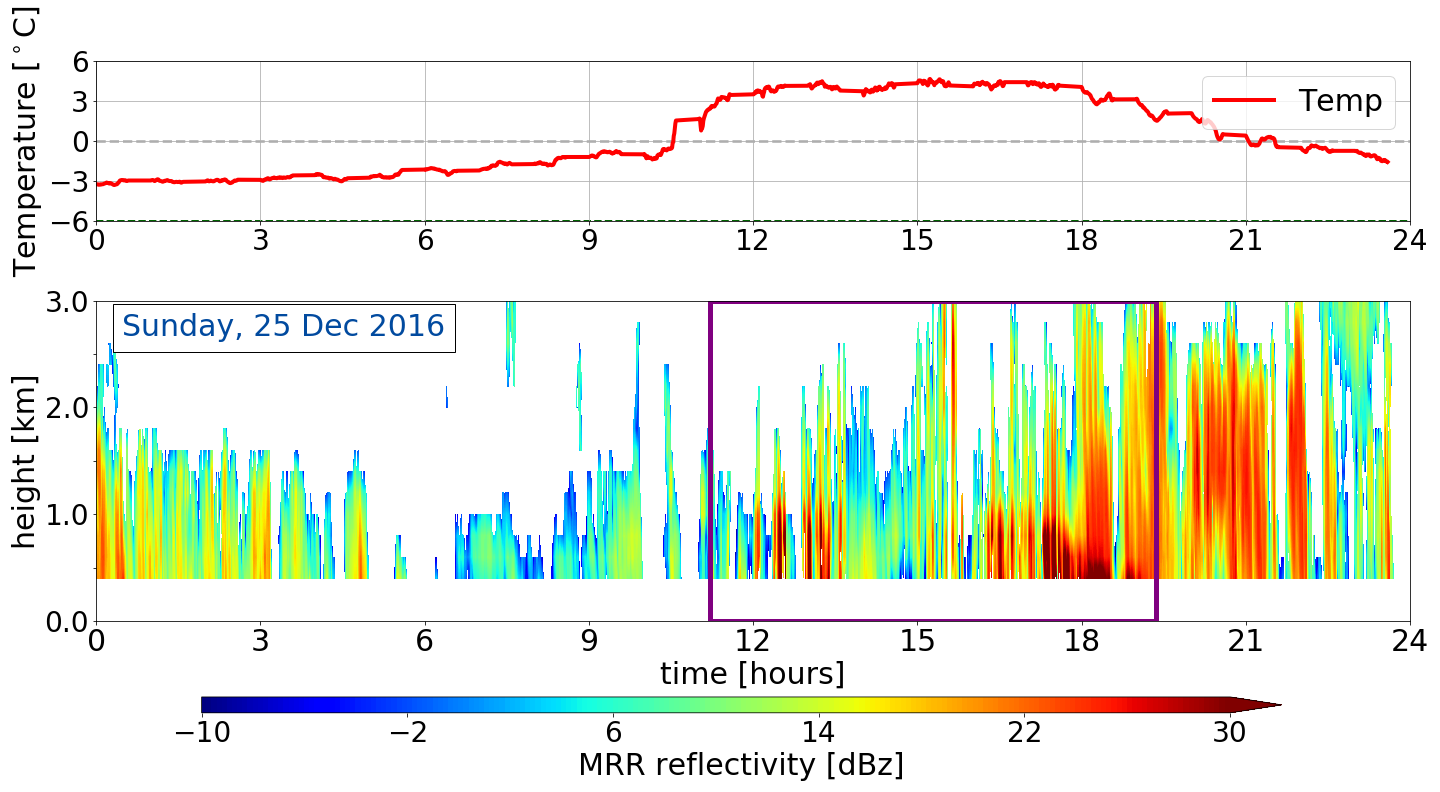
\includegraphics[width=\textwidth]{./fig_MRR/MRR_sfcT_20161225}
	%	\end{subfigure}
	\caption{A priori temperature dependence within the optimal estimation retrieval for an all day precipitation event on \SI{25}{\dec}. The upper panel shows the surface a priori guess, $T_{ap}$, measured at the Haukeliseter site. The lower panel presents the reflectivity measure by the MRR. Additionally, indicates the purple frame the time, where the MRR reflectivity was larger than \SI{-10}{\dB Z} and surface temperatures less than \SI{2}{\celsius} }\label{fig:MRR_sfcT}
\end{figure}
%%%%%%%%%%%%%%%%%%%%%%%%%%%%%%%%%%%%%%%%%%%%%%%%%%%%%%%%%%%%%%%%%%%%%%%%%%
To achieve vertical profiles of snowfall from MRR different steps and assumptions are done in the here presented snowfall retrieval. From one of the lower levels, the snowfall rate at the surface can be estimated. The retrieval is only performed for profiles, which are likely to have observed snow, where most retrievals use rain. In previous studies relationships between reflectivity and snowfall have been developed. Even if the PSD of ice particles is known, different crystal shapes led to different results. Snow densities vary significantly from storm to storm, where small particles are still Rayleigh scattered, and larger particles non-Rayleigh scattered \citep{gunn_microwave_1954}. 
\\
To obtain the likelihood of present snow a reflectivity threshold of \SI{- 15}{\decibel Z} is used. This threshold is similar to the one used in \cite{wood_level_2013}, where it states that light liquid precipitation is related to \SI{- 10}{\decibel Z} \citep{stephens_properties_2007}. \cite{wood_estimation_2011} compared the reflectivity in the lowest bin and adjacent bin and found, that the reflectivity above \SI{-15}{\dB Z} are not influenced by ground clutter.
\newline
The Haukeliseter measurement site is equipped with a weather mast, measuring the air temperature every minute at two meter height (compare \Cref{fig:MRR_sfcT}, upper panel). 
%
Since the MRR measures above \SI{300}{\metre} and only temperature measurements at the surface exists, a priori temperature ($T_{a}$) is assumed to be similar to the observed near-surface air temperature. Using a moist adiabatic lapse rate of $dT/dz = \SI{5}{\kelvin\per\km}$ gives $T_{a}$ in each layer. 
Assuming snow exists at temperature measurements up to a threshold of \SI{2}{\celsius}, validated by \cite{liu_g._deriving_2008} who analysed present weather reports to find the distinction between liquid and solid precipitation.\\
The purple line in the lower panel of \Cref{fig:MRR_sfcT} represents the time frame during \SI{25}{\dec}, where the MRR reflectivity is less than \SI{- 15}{\decibel Z}, and a priori temperature passes the \SI{2}{\celsius} limit at the surface.  


\subsection{Size distribution} \label{sec:size_dist}
To determine the snowfall rate at the surface an exponential particle size distribution (PSD) is needed. 
\begin{align}
	n(r) & = N_{0} \exp\left(-\lambda r\right) \qquad [ \SI{}{\per\cubic\metre\per\mm} ] \label{eq:num_dens}
\end{align}
where $\lambda$ represents the PSD slope parameter and $N_{0}$ the number concentration. $r$ is the particle maximum dimension evaluated from the 2D-scattering model for branched 6-arm spatial particles with porosities for reflectivity measurements at \SI{24}{\giga\Hz} (see \Cref{app:scat_scheme}).
%exponential particle size distribution (PSD) \\
%	$$ \qquad \text{$D$ from B6 scattering model}$$
%	$$\lambda = 10^{perturbuation}$$ %\\
%   %$$N_0 = 10^{perturbation}$$
%The slope parameter and the number density in \Cref{eq:num_dens} varies with height with the help of the following logarithmic assumptions \textcolor{red}{In vsnow_hmrr.pro: DEFINE A PRIORI PSD INFO (LOG FORM) THROUGH WOOD TEMPERATURE PARAMETERIZATION}.
\\
Since $T_{a}$ varies with a moist adiabatic lapse rate in each layer bin the slope parameter and the number concentration in \Cref{eq:num_dens} are changing too. \cite{wood_estimation_2011} showed a linear fit between $\log(\lambda)$ and the a priori temperature, respectively $\log(N_0)$ and the a priori temperature.
Using $T_{a}$ in \SI{}{\celsius} for each layer bin the following logarithmic assumption is used, to define the slope parameter and the number concentration.
\begin{align}
	\log(\lambda) & = -0.03053 \cdot T_{ap} - 0.08258  \label{eq:lambda} \qquad [ \log(\SI{}{\per\mm}) ]\\
	\log(N_0) & = -0.07193 \cdot T_{ap} +2.665  \qquad [ \log(\SI{}{\per\cubic\metre\per\mm})]
	\label{eq:N0}
\end{align}
% \item \citep{wood_level_2013}: state is described by the exponential size distribution parameters $N_0$ and $\lambda$. Values for $N_0$ may range over several order of magnitude, so $log(N_0$) is retrieved instead. $log(\lambda$) is retreived since they are less skewed and $\lambda$ was strongly non-Gaussian. \textcolor{red}{where is this equations from?}\\
To achieve the state vextor $\mathbf{x}$ of unknown microphysical properties, the log-transformed values are taken.
\begin{align}
	\mathbf{x} & = \begin{bmatrix}
		log(\lambda)_0 	\\
		\vdots 			\\
		log(\lambda)_{\text{nlayer}} 	\\
		log(N_0)_0		\\
		\vdots			\\
		log(N_0)_{\text{nlayer}}		
	\end{bmatrix} \qquad \text{nlayer} = 14
	\label{eq:snow_prop}
\end{align}
The log-transformed equation is useful, since the results from C3VP were similar to other observations. The study showed, that $N_0$ ranges over several order of magnitude as well as $\lambda$ was non-Gaussian for the snow events \cite{wood_estimation_2011}.



\subsection{Snowfall retrieval scheme}\label{sec:ret_scheme}
The optimal estimation method is based on Gaussian statistics. Minimizing the scalar cost function, $\Phi$ for the snowfall properties, $\mathbf{x}$. The cost function weights the difference between the observed reflectivity and the simulated measurements as well as the difference between the estimated and a priori guess. %A forward model $F(\mathbf{x})$ relates unknown snowfall parameters $\mathbf{x}$ to radar observations $y$ and approximates the true physical state between them \citep{wood_estimating_2014,cooper_variational_2017}. 
\\
Scalar cost function:
\begin{equation}
\begin{split}
\Phi(\mathbf{x},y,a) = & (y- F(\mathbf{x}))^T \mathbf{S}_y^{-1} 			(y-F(\mathbf{x})) \\
&+(\mathbf{x}-a)^T \mathbf{S}_{a}^{-1} (\mathbf{x}-a)
\end{split} \label{eq:scalar_cost_fct}
\end{equation}
where, $\mathbf{x}$, vector of retrieved snowfall properties (\Cref{eq:snow_prop}); $y$, vector of observation (MRR reflectivity) ; $a$, vector of the a priori guess (temperature dependent); $\mathbf{S}_a$, a priori error covariance matrix; $\mathbf{S}_y$, measurement error covariance matrix. The forward model $F(\mathbf{x})$, presented in \Cref{sec:forward_model} relates unknown snowfall parameters $\mathbf{x}$ to radar observations $y$ and approximates the true physical state between them \citep{wood_estimating_2014,cooper_variational_2017}.
%
% a priori: $$
% 		\mathbf{S}_a = \begin{bmatrix}
%        0.133 	& 0 	& \dots & 0 		& 0         \\%[0.3em]
%        0		& 0.133 & \dots	& 0 		& 0		 \\
%        \vdots 	& \vdots& \vdots& \ddots 	& \vdots \\
%        0		& 0		& \dots	& 0.95 		& 0 \\
%        0 		& 0		& \dots & 0 		& 0.95
%      \end{bmatrix} $$
\\
$\mathbf{S}_a$ links the uncertainties of the PSD information and the surface temperature differences. The diagonal matrix elements in $\mathbf{S}_a$ are equal to \numlist{0.133;0.95} for the particle slope parameter and the number concentration, respectively as from  Eq. 7.35 and 7.36 in \cite{wood_estimation_2011}. \\
% $$\mathbf{S}_y = \begin{bmatrix}
%        6.25 	& 0 	& \dots & 0 		& 0         \\%[0.3em]
%        0		& 6.25 & \dots	& 0 		& 0		 \\
%        \vdots 	& \vdots& \vdots& \ddots 	& \vdots \\
%        0		& 0		& \dots	& 6.25		& 0 \\
%        0 		& 0		& \dots & 0 		& 6.25
%      \end{bmatrix} $$ 
$\mathbf{S}_y$ characterises the the uncertainties associated with the measurements and the error in the forward model. This study uses for the diagonal matrix elements $2.5^2$ \textcolor{red}{UNIT!? based on the study from CITATION. BECAUSE.}
\\
% sensitivity matrix: K \\
% 	$$\pm perturbation = \hat{x} \cdot \left(1 \pm \frac{0.2}{100}\right)$$ \\
% 	perform Forward model \\
% 	matrix of Kernel functions, Jacobian of forward model with respect to the state vector 
% 	$$fn_{i,j} = \frac{y_{max_j} - y_{min_j}}{+ perturbation_i - (- perturbation_i)}$$
% 	$$\mathbf{K}(i,j) = \begin{bmatrix}
% 		fn_{0,0} 	& fn_{1,0} 		& \ldots & fn_{m-1,0} \\
%         fn_{0,1} 	& fn_{1,1}	 	& \ldots & fn_{m-1,1} \\
%         \vdots	 	& \vdots		& \ddots & \vdots 	\\
%         fn_{0,n-1} 	& fn_{1,n-1}	& \ldots & fn_{m-1,n-1}
% 	\end{bmatrix}$$
%
% covariance of solution $\hat{x}$ at convergence
%    $$$$
\textcolor{red}{I don't understand the next steps and if it is still the same $\mathbf{x}$?!} 
\\
At convergence is the error covariance of the retrieved state vector $\mathbf{S}_x$
\begin{align}
	\mathbf{S}_x & = \left( \mathbf{S}_a^{-1} + \mathbf{K}^T \mathbf{S}_y^{-1} \mathbf{K} \right)^{-1}
\end{align}
which follows for $\mathbf{x}$
\begin{align}
	\mathbf{x} & = \underbrace{\left( \mathbf{S}_a^{-1} + \mathbf{K}^T \mathbf{S}_y^{-1} \mathbf{K} \right)^{-1} }_\text{$\mathbf{S}_x$} \left( \mathbf{S}_a^{-1} a + \mathbf{K}^T \mathbf{S}_y^{-1} \left(y - F(\mathbf{x}) + \mathbf{K} \mathbf{x} \right)  \right)
\end{align}
%\textcolor{red}{\cite{wood_level_2013}: 'As a diagnostic test of the results, a $\chi^2$ statistic is calculated using the retrieved state vector.}
The Jacobian matrix, $\mathbf{K}$, represents the sensitivity matrix of the perturbed result of the forward model. The true state $\mathbf{x}$ is perturbed by \SI{\pm 0.2}{\percent} and thus $\mathbf{K}$ represents the relation between simulated values to the true state.  \textcolor{red}{Why are we perturbing it?}
\begin{align}
	\mathbf{K}(\mathbf{x}) & = \frac{\partial y}{\partial \mathbf{x}} =
	\begin{bmatrix}
		\frac{\partial y_0}{\partial \mathbf{x}_0} & 
		\frac{\partial y_0}{\partial \mathbf{x}_1}  & 
		\ldots & 
		\frac{\partial y_0}{\partial \mathbf{x}_{2\,\text{x\,nlayer}}} \\[0.3em]
		\vdots & \vdots & \ddots & \vdots \\[0.3em]
		\frac{\partial y_{\text{nlayer}}}{\partial \mathbf{x}_0} &
		\frac{\partial y_{\text{nlayer}}}{\partial \mathbf{x}_1} &
		\ldots &
		\frac{\partial y_{\text{nlayer}}}{\partial \mathbf{x}_{2\,\text{x\,nlayer}}}
	\end{bmatrix} % Eq. 3.6 in \cite{wood_estimation_2011}
	\label{eq:Kmatrix}
\end{align}
Usually, is $\mathbf{K}$ not diagonal \citep{wood_estimation_2011}, hence it is a mix of the true state and the a priori guess and the influence from them can be estimated. 
The closer $\mathbf{K}$ is diagonal, the more is $\mathbf{x}$ determined by the real observed and a priori values. If the limit of the partial derivative is close to unity, the retrieved value $\mathbf{x}$ is its true state \citep{wood_estimation_2011}. \\
\\
\textcolor{red}{mmmh? What exactly are we doing here?}
Test the if convergent:
\begin{align}
	\hat{x} & = \left( \mathbf{x} - F(\mathbf{x}) \right)^T \mathbf{S}_x^{-1} \left(\mathbf{x} - F(\mathbf{x}) \right)
\end{align}
only if $\hat{x}$ is smaller than \num{2} it is a 'good' retrieval. 
\\
To test the result of $\mathbf{x}$ a $\chi^2$ test is performed at the convergence of $\mathbf{S}_x$.
%
\begin{equation}
\begin{split}
\chi^2 = & \left( F(\mathbf{x}) - y  \right) \mathbf{S}_y^{-1} \left( F(\mathbf{x}) - y \right)^T \\
& + \left( \mathbf{x} - a \right)^T \mathbf{S}_a^{-1} \left( \mathbf{x} - a\right). 
\end{split}
\label{eq:chi}
\end{equation}
%
The first term in \Cref{eq:chi} measures the part of $\chi^2$ related to the noise of the forward model, and the second part the relation to the state vector. Thus the second term describes the accuracy of the quantities within the reflectivity and temperature measurements \citep{rodgers_inverse_2000}.
% error contribution 
Furthermore, are the error contribution from the reflectivity measurement uncertainty, $\mathbf{S}_{y_\epsilon}$, and the uncertainty of the a priori values, $\mathbf{S}_{a_\epsilon}$ estimated. \textcolor{red}{Where comes this formulas from? Is the $\mathbf{D}_y$ the $\mathbf{K}_b$ in Eq. 15 in \cite{wood_characterization_2013}? How to interpret?}
%
\begin{align}
	\mathbf{D}_y  & = \mathbf{S}_x \mathbf{K}^T \mathbf{S}_y^{-1} %\hspace{4cm} 
	& \mathbf{S}_{y_\epsilon} & = \mathbf{D}_y \mathbf{S}_y \mathbf{D}_y^T \\
	\mathbf{D}_a & = \mathbf{S}_x \mathbf{S}_a^{-1} %\hspace{4cm} 
	& \mathbf{S}_{a_\epsilon} & = \mathbf{D}_a \mathbf{S}_a
\end{align}
The diagonal of $\mathbf{S}_{y_\epsilon}$ or $\mathbf{S}_{a_\epsilon}$ is a first estimate of the retrieval noise related to the observations \citep{rodgers_inverse_2000}. Uncertainties in $\mathbf{S}_{a_\epsilon}$ occur because of the variability in $T_a$ and similar for $\mathbf{S}_{y_\epsilon}$ due to measurement errors from the MRR.
%
%
\newpage
\subsection{Forward model}\label{sec:forward_model}
% %%% image forward problem %%%%%%%%%%%%%%%%%%%%%%%%%%%%%%%%%%%%%
% !TeX spellcheck = en_GB
\begin{wrapfigure}[17]{r}{0.44\textwidth}
	\vspace{-\normalbaselineskip}
	\centering
	\begin{subfigure}[b]{0.4\textwidth}
		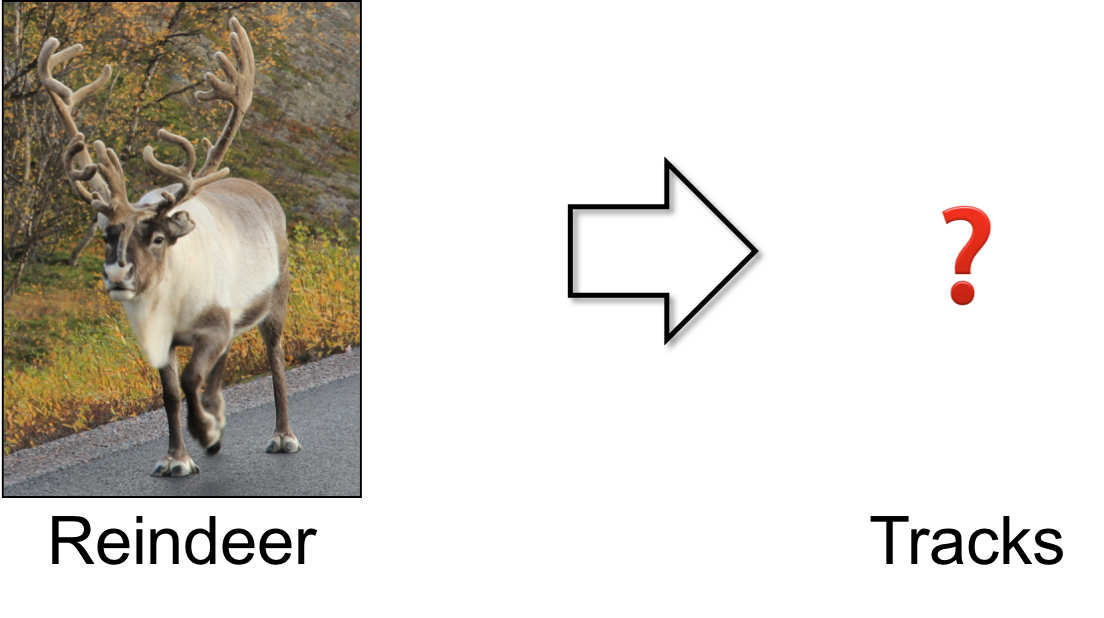
\includegraphics[trim={0cm, 0cm, 0cm, 0cm},clip,width=\textwidth]{./fig_instruments/Forward_problem.png}
		\caption{Forward problem.}\label{fig:dragon:forward}
	\end{subfigure}
	
	\begin{subfigure}[b]{0.4\textwidth}
		
\includegraphics[trim={0cm, 0cm, 0cm, 0cm},clip,width=\textwidth]{./fig_instruments/Inverse_problem.png}
		\caption{Inverse problem.}\label{fig:dragon:inverse}
	\end{subfigure}
	\caption{\protect\subref{fig:dragon:forward}: Forward problem, relationship between parameter of interest (reindeer) and the unknown parameter of measurements (tracks). \protect\subref{fig:dragon:inverse}: An inverse problem when the parameter of measurements is known, but the parameter of interest is not \citep{stephens_remote_1994}.}\label{fig:dragon}
	\vspace{-\normalbaselineskip} 
\end{wrapfigure}


%%%%%%%%%%%%%%%%%%%%%%%%%%%%%%%%%%%%%%%%%%%%%%%%%%%%%%%%%%%%%%%%%%%%%%%%%%
Forward model defines a relationship between the radar observations and the retrieved state vector $\mathbf{x}$. It is difficult to find the properties of the atmosphere by using observations due to unknown parameters influencing the measurement. \\
\cite{stephens_remote_1994} described the forward problem in the manner that a Dragon represents the known source, observations \Cref{fig:dragon}. The amount of received radiation lost during the transmittance to the sensor is unknown, the Tracks in \Cref{fig:dragon}. The forward model will help to find simulated observations before the attenuation took place and give information about the tracks of the dragon.  
\\
The knowledge about the a priori parameters and related covariances, as well as $\mathbf{x}$, are used to minimize \Cref{eq:scalar_cost_fct}. The values of $\mathbf{x}$ are found by Newtonian iteration \cite[Eq. 5]{wood_estimating_2014}.
\newline
The snow water content in each layer is estimated from the knowledge of the snow particle mass-dimension relationship in \Cref{app:scat_scheme}, and a PSD related to slope parameter and number concentration (\Cref{eq:num_dens,eq:lambda,eq:N0}). % Snow water content  in each layer 
\begin{align}
	\text{SWC} & = \int_{r_{min}}^{r_{max}} m(r) n(r) dr \qquad [\SI{}{\gram\per\cubic\metre}] \label{eq:SWC}
\end{align}
To achieve a relationship between the reflectivity and the snowfall amount one needs to account for attenuation in the atmosphere. Using the previously calculated PSD (\Cref{eq:num_dens}) the backscattering cross-section $\sigma_{bk}$, one can estimate the reflectivity for Rayleigh approximated, singly-scattered non-attenuated ice particles \citep{lecuyer_estimation-based_2002,kulie_utilizing_2009,wood_microphysical_2015}. The Rayleigh approximation assumes, that $2\pi r/\lambda \ll 1$, where $\lambda$ the wavelength of incident radiation.
% singly-scattered non-attenuated reflectivity
\begin{align}
	\eta_{bk} & = \int_{r_{min}}^{r_{max}} n(r) \sigma_{bk} dr \qquad [\SI{}{\per\metre}] \nonumber \\
	Ze^{ss,na} & = \frac{\Lambda^4}{\left\| K_w \right\|^2 \pi^5} \eta_{bk} \qquad \textcolor{red}{[\SI{}{\mm^6\metre^{-3}}]} \label{eq:singleZ}
\end{align}
% $\ldots$ snow backscatter coefficient
where, $\Lambda$ is the wavelength of the radar; $\left\| K_w \right\|^2$ is the complex refractive index of water and varies between \numlist{0.91;0.93} for wavelength between \SIlist{0.01;0.10}{\metre} and is independent of temperature. It also exists a  complex refractive index for ice $\left\| K_i \right\|^2$, which is \SI{0.18}{}. This is valid for a density of \SI{0.917}{\gram\per\cubic\cm} and is independent of temperature and of wavelength in the microwave region \citep{doviak_doppler_1993}. In this work  $\left\| K_w \right\|^2 = 0.93$ is chosen, \textcolor{red}{BECAUSE???}. 
\\
The singly-scattered reflectivity has to be corrected for attenuation in the layers above the actual layer. According to Beer's law is in a homogeneous medium one way transmission assumed. 
% account for attenuation
% homogeneous medium $\Rightarrow$ one way transmission, Beer's law
\begin{align}
	\frac{I_{\lambda}}{I_{\lambda_0}} & = \exp \left[ - \int_0^s \beta_{ext} ds'\right] \label{eq:Beer}
\end{align}
where $s$ is the path length through the medium. The transmissivity $I_{\lambda}/I_{\lambda_0}$ is the relation of survived radiation through extinction in the atmosphere with the snow extinction coefficient $\beta_{ext}$
\begin{align}
	\beta_{ext} & = \int_{r_{min}}^{r_{max}} n(r) \sigma_{ext} dr \qquad [\SI{}{\per\metre}] \label{eq:bext}
\end{align}
The extinction coefficient is the sum of absorption and scattering in the atmosphere followed from the extinction cross-section $\sigma_{ext} = \sigma_{abs} + \sigma_{scat}$, \citep{lohmann_introduction_2016,lamb_physics_2011}. \textcolor{red}{\cite[Eq. 12.1 and more][]{lohmann_introduction_2016}} \\
%singly-scattered attenuated reflectivity 
Following \Cref{eq:singleZ,eq:Beer,eq:bext} the singly-scattered attenuated reflectivity $Ze^{ss, a}$ is
\begin{align}
	Ze^{ss, a} & = Ze^{ss, na} \cdot \frac{I_{\lambda}}{I_{\lambda_0}} \qquad \textcolor{red}{[\SI{}{\mm^6\metre^{-3}}]} \label{eq:sing_scatt_att_Z}
\end{align}
% multiply-scattered attenuated reflectivity 
% \cite{matrosov_s._y._influence_2009} found that in heavy snow conditions the multiply-scattered attenuated reflectivity lies between the singly-scattered attenuated and non-attenuated reflectivities \citep[compare Fig. 3.3 in][]{matrosov_s._y._influence_2009}. Therefore, is as in \cite{wood_level_2013} the multiply-scattered attenuated reflectivity, $Ze^ms$, approximated as geometric mean.
% \begin{align}
% 	Ze^ms & = \sqrt{Ze^{ss,na} \cdot Ze^{ss,a}} \qquad [\SI{}{\dB Z}]
% \end{align}
% $\Rightarrow$ simulated reflectivities from forward model 
That follows with the use of radiative transfer equations for the simulated reflectivity from the forward model, $F(\mathbf{x})$ in \Cref{eq:scalar_cost_fct}, after the transformation with \Cref{eq:Ze}
\begin{align}
	F(\mathbf{x}) & = \begin{bmatrix} 
		Ze^{ss,a}_1 \\
		\vdots \\
		Ze^{ss,a}_{nlayer}
	\end{bmatrix} \qquad [\SI{}{\decibel Z}]. \label{eq:forward_model}
\end{align}


\begin{itemize}
	\item \textcolor{red}{not really using the following - What to do with it?}
	\item \textcolor{red}{total number concentration} \\
	$$n_{tot} = \int_{r_{min}}^{r_{max}} n(r) dr \qquad [\SI{}{\per\cubic\metre}]$$ 
	\item $\ldots$ \textcolor{red}{??? }
	
\end{itemize}



\subsection{Snowfall rate at the surface}
%
% fall speed assumption:
To achieve snowfall rates at the surface, the snow water content (\Cref{eq:SWC}) has to be transformed. The use of an assumed particle fall speed of $V = \SI{0.85}{\mPs}$ and the retrieved SWC (\Cref{eq:SWC}) gives the snow mass flux $J_{snow} = \text{SWC} \cdot V$ in [\SI{}{\kilogram\per\square\metre\per\second}]. \textcolor{red}{Why did we use this fall speed? Where does this assumption come from? Similar as \cite{cooper_variational_2017} Eq. 4?} 
% snow mass flux
To compare retrieved snow fall rates to double fence measurements and the forecast model output, the precipitation amount at the surface is calculated. 
\begin{align}
	P = J_{snow} \times \num{e-3} \cdot \left(\SI{3600}{\second} \cdot24 \right) \qquad [\SI{}{\mm\per\day}]
\end{align}
The precipitation amount at the surface, presented in \Cref{ch:Res}, are taken to be equal to the values at the snow layer in \SI{800}{\metre}. The use of the values at \SI{800}{\metre} is due to the small increase of reflectivity (ground clutter) in the bottom layers and would follow more observed snow. 
%
\begin{itemize}
	\item \textcolor{red}{Not sure what to do with this!}
	\item The error from the retrieved state vector $\mathbf{x}$ is calculated
	$$\pm \mathbf{S}_{x_{err}} = \mathbf{x} \pm \mathbf{S}_x$$ 
	$$equiv_{err} = \frac{1}{2} \left( \frac{\abs{\text{SWC}(- \mathbf{S}_{x_{err}} ) - \text{SWC} (+ \mathbf{S}_{x_{err}}) }}{ \text{SWC}(- \mathbf{S}_{x_{err}})} + \frac{\abs{ \text{SWC}(- \mathbf{S}_{x_{err}}) - \text{SWC}(- \mathbf{S}_{x_{err}}) }}{ \text{SWC}(- \mathbf{S}_{x_{err}})} \right)$$
\end{itemize}








%%%%%%%%%%%%%%%%%%%%%%%%%%%%%%%%%%%%%%%%%%%%%%%%%%%%%%%%%%%%%%%%%%%%%%%%%%
%%%%%%%%%%%%%%%%%%%%%%%%%%%%%%%%%%%%%%%%%%%%%%%%%%%%%%%%%%%%%%%%%%%%%%%%%%
% %%% ***************** CHAPTER MEPS ***************** %%%
% !TeX spellcheck = en_GB
\section{MetCoOp Ensemble Prediction System}
MEPS (MetCoOp Ensemble Prediction System) was newly operational at Met-Norway when the extreme weather occurred in Norway. Comparing model data with actual observations helps to verify the agreement between model prediction and ground-based measurements. 
\\
AROME-MetCoOp was operational from March 2014 until November 2016, when it was replaced with an ensemble prediction system (EPS) based on AROME-MetCoOp.
MEPS is used as weather forecast at the Norwegian Meteorological Institute, the Swedish Meteorological and Hydrological Institute (SMHI) and the Finnish Meteorological Institute (FMI), \citep{muller_arome-metcoop:_2017, koltzow_metcoop_2017}.
%%%%%%%%%%%%%%%%%%%%%%%%%%%%%%%%%%%%%%%%%%%%%%%%%%%%%%%%%%%%%%%%%%%%%%%%%%
%%%%%%%%%%%%%%%%%%%%%%%%%%%%%%%%%%%%%%%%%%%%%%%%%%%%%%%%%%%%%%%%%%%%%%%%%%
%%%%%%%%% MEPS %%%%%%%%%%%%%%
\subsection{AROME - MetCoOP}
In principle, MEPS is a short-term weather forecast consisting of a ten ensemble member  forecast system with \SI{66}{\hour} prediction time and a horizontal resolution of \SI{2.5}{\km} and 65 vertical levels. One of the members is the deterministic forecast where the other nine present the perturbed state of the deterministic forecast. The initialisation of each member is performed at \SIlist{00;06;12;18}{\UTC} \citep{metcoop_wiki_description_2017}.
\\ 
Forecast data saved for the deterministic and first ensemble member have a time resolution of one hour for \SI{66}{\hour}. The other eight members have values every three hours for up to \SI{48}{\hour} forecast time.
%\\
%%% image MEPS resolution %%%%%%%%%%%%%%%%%%%%%%%%%%%%%%%%%%%%%
% !TeX spellcheck = en_GB
% \begin{figure}[t]
% 	\centering
%     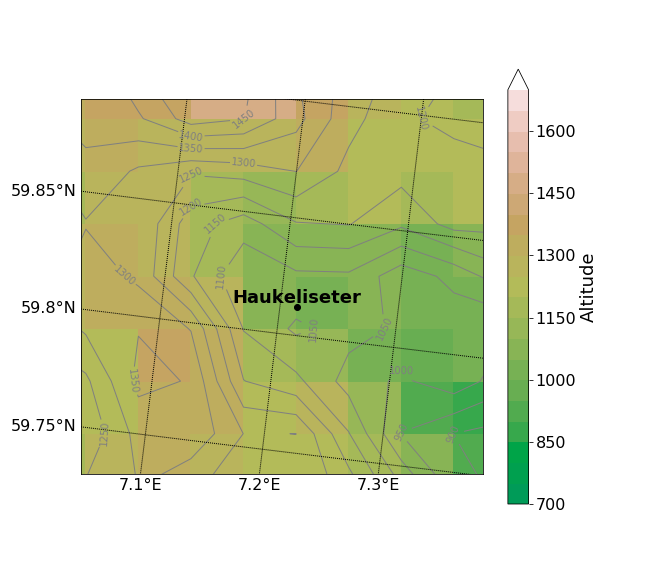
\includegraphics[trim={.3cm 2.2cm 1.8cm 2.4cm},clip,width=\textwidth]{./fig_Norway/MEPS_elevation_Haukeli}
%         \caption{}\label{fig:meps:site}
% \end{figure}

% \begin{wrapfigure}[14]{r}{0.55\textwidth}
% 	\vspace{-\normalbaselineskip}
% 	\centering
% 	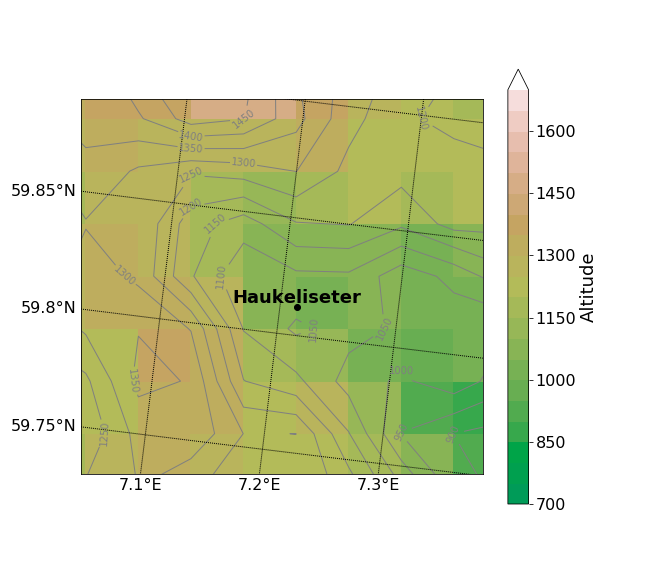
\includegraphics[trim={.3cm 2.2cm 1.8cm 2.4cm},clip,width=0.54\textwidth]{./fig_Norway/MEPS_elevation_Haukeli}
% 	%	\vspace{-10pt}
% 	\caption{Representation of the topography around measurement site Haukeliseter in MEPS. Contours and shading present the elevation of the grid cells.}\label{fig:meps:site}
% 	\vspace{-\normalbaselineskip}
% \end{wrapfigure}

% !TeX spellcheck = en_GB
\begin{figure}[ht!]
	\centering
    \begin{subfigure}[b]{0.53\textwidth}
    	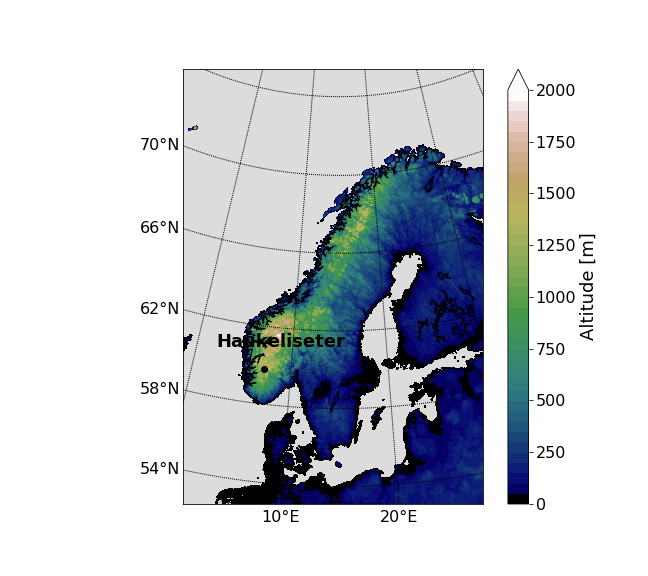
\includegraphics[trim={4.cm 1.8cm 0cm 2.cm},clip,width=1.05\textwidth]{./fig_Norway/Norway_elevation_MEPS}
        \caption{}\label{fig:meps:Norway}
    \end{subfigure}
    \begin{subfigure}[b]{0.46\textwidth}
        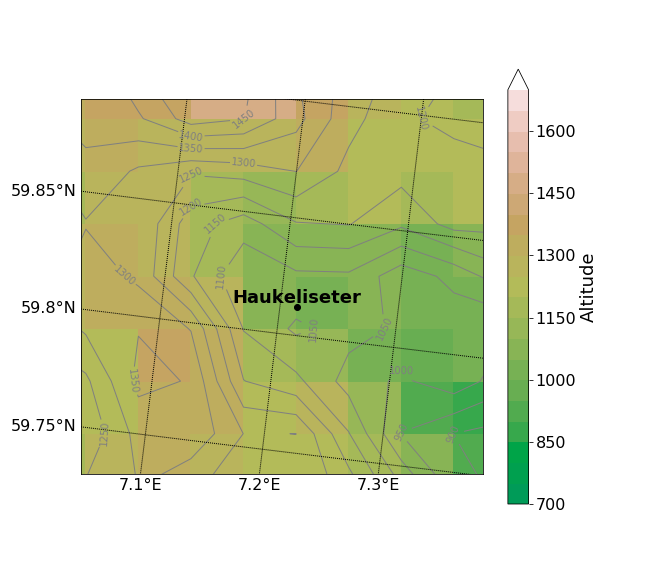
\includegraphics[trim={.3cm 2.2cm 1.8cm 2.4cm},clip,width=\textwidth]{./fig_Norway/MEPS_elevation_Haukeli}
        \caption{}\label{fig:meps:site}
      \end{subfigure}
	\caption{\protect\subref{fig:meps:Norway}: Elevation map of MEPS model domain. \protect\subref{fig:meps:site}: Representation of the topography around the measurement site Haukeliseter in MEPS. Contours and shading present the elevation of the grid cells.}\label{fig:meps_site}
\end{figure} 
%%%%%%%%%%%%%%%%%%%%%%%%%%%%%%%%%%%%%%%%%%%%%%%%%%%%%%%%%%%%%%%%%%%%%%%%%%
\noindent
\Cref{fig:site:Norway} shows the MEPS model domain and its elevation as it was operational for December 2016. It covers the Nordic Countries including open water such as the Atlantic Ocean, the North and the Baltic Sea. A representation of the horizontal resolution zoomed on the Haukeliseter site is shown in \Cref{fig:meps:site}. Haukeliseter is surrounded by a complex terrain with mountains up to \SI{1500}{\metre} no the west and the north and the more open terrain to the south-east.
\\
The centre of the model is approximately at \ang{63.5}\,N, \ang{15}\,E. 
The horizontal grid points are projected on a Lambert projection to receive the same area size of each grid cell. 
The outer, parent grid is the ECMWF-IFS model (European Centre for Medium-Range Weather Forecasts Integrated Forecasting System) with a horizontal resolution of \SI{9}{\km} \citep{homleid_verification_2016}. The ECMWF-IFS forecasts are used \SI{6}{\hour} prior to the actual cycle in MEPS.
\\
Vertical hybrid coordinates are terrain-following and are mass-based, \citep{muller_arome-metcoop:_2017}. How the vertical hybrid coordinates are transformed into layer thickness or height is described in \Cref{sec:layer_thickness}. Furthermore, MEPS underlies non-hydrostatic dynamics, \cite{metcoop_wiki_description_2017}.
\\
The representation of snow is covered by a modification of the three-class ice parametrization (ICE3) scheme. Where liquid-phase processes are separated from slow ice-phase processes and described in \Cref{sec:MesoNH}. To model the snow cover an one-layer atmosphere model scheme is implemented. This includes three variables such as: snow water equivalent (SWE), snow density, and snow albedo \citep{muller_arome-metcoop:_2017}.
\\
As synoptic observations are included in the model the snow-depth predictions underlay a special performance. Observations of snow-depth are only available at \SIlist{06;18}{\UTC}, therefore is the snow analysis only performed twice daily \citep{muller_arome-metcoop:_2017, homleid_verification_2016}. 
%The MEPS forecasting system consist of 1+9 members where each of the perturbed members perform an initialization of \SI{66}{\hour} at \SIlist{00;06;12;18}{\UTC} \citep{metcoop_wiki_description_2017}. 
%\\
%For more detailed information to the model the reader is referred to \cite{muller_arome-metcoop:_2017} and \cite{wiki_description_2017} and its references therein.
%
%%%%%%%%%%%%%%%%%%%%%%%%%%%%%%%%%%%%%%%%%%%%%%%%%%%%%%%%%%%%%%%%%%%%%%%%%%
%%%%%%%%%%%%%%%%%%%%%%%%%%%%%%%%%%%%%%%%%%%%%%%%%%%%%%%%%%%%%%%%%%%%%%%%%%
%%%%%%%%% MESONH %%%%%%%%%%%%%%
\subsection{Meso-NH and the ICE3 scheme} \label{sec:MesoNH}
The physical parametrization within AROME is based on the French research communities' mesoscale non-hydrostatic atmosphere model (Meso-NH). The microphysical scheme in the Meso-NH atmospheric simulation system is based on the ICE3 scheme. The purpose of the scheme is to model as correctly as possible the ice phase in the atmosphere \citep{pinty_mixed-phased_1998}. \cite{mccumber_comparison_1991} concluded from their case study, that at least three different ice categories are necessary to cover most precipitation but that applications might be case specific. 
According to the \cite{meteo_france_meso-nh_2009} documentation, the ice phase microphysical scheme must include: 
\begin{itemize}
	\item [\textbf{r$_i$:}] pristine ice phase  
	\item [\textbf{r$_s$:}] snowflake type from lightly rimed large ice crystals or dry clusters, and
	\item [\textbf{r$_g$:}] heavily rimed crystals, such as graupel, frozen drops or hail
\end{itemize}
% %%% table ice parameters %%%%%%%%%%%%%%%%%%%%%%%%%%%%%%%%%%%%%
% % % !TeX spellcheck = en_GB
\begin{table}[h]
	\begin{center}
		\caption{Characterization parameters from primary ice (r$_i$), snowflakes (r$_s$) and rimed crystals (r$_g$). Values are based on the references in \cite{meteo_france_meso-nh_2009} and in \cite{pinty_mixed-phased_1998}. }\label{tab:ice_parameter}
		\begin{tabular}{l|c|c|c}
			\hline \hline
			& \textbf{r$_i$}& \textbf{r$_s$}& \textbf{r$_g$} \\ \hline\hline
			$\alpha$, $\nu$ & \num{3.3}		& \num{1.1}			& \num{1.1} \\ \hline
			$a$				& \num{0.82}	& \num{0.02}		& \num{196} \\ 
			$b$				& \num{2.5}		& \num{1.9}			& \num{2.8} \\ \hline
			$c$				& \num{800}		& \num{5.1}			& \num{124} \\ 
			$d$				& \num{1.0}		& \num{0.27}		& \num{0.66} \\ \hline
			$C$				&				& \num{5}			& \num{5e5} \\
			$x$				&				& \num{1}			& \num{-0.5} \\
			\hline \hline
		\end{tabular}
	\end{center}
\end{table}
% %%%%%%%%%%%%%%%%%%%%%%%%%%%%%%%%%%%%%%%%%%%%%%%%%%%%%%%%%%%%%%%%%%%%%%%%%%
Within the ICE3 scheme no distinction between hail and graupel exists and therefore is the physical discrimination in the growth mode of graupel and hail is neglected. \\
To achieve snow water content within MEPS the total number concentration, slope parameter, mass diameter and  the particle size distribution have to be determined. 
According to \cite{caniaux_numerical_1994} follows the particle size distribution the Marshall-Palmer distribution similar to \Cref{eq:num_dens}. The goal is to use a varying number concentration $N_0$ dependent on the ice category. The study has shown that $N_0$ can be assumed with
\begin{align}
	N_0 & = C \lambda^x  \label{eq:model_N0}
	\\
	\log_{10}C & = -3.55x + 3.89  \nonumber
\end{align}
where $C$ and $x$ depend on the ice category and represent the relation between each other in \Cref{eq:model_N0}. 
\\
The ice water content for primary ice, snowflakes and rimed crystals is then be assumed to be similar to \Cref{eq:SWC}, but the integration limits range from zero to infinity and mass, and particle size distribution are dependent on the diameter of the particle. The mass diameter and particle size distribution (\Cref{eq:mass_diameter,eq:PSD_MEPS}) are represented depending on the ice category shown in \Cref{tab:ice_parameter}
\begin{align}
	m(D) & = aD^b 	\label{eq:mass_diameter} \\
	n(D) & = N_0 g(D)	\label{eq:PSD_MEPS}
\end{align}
and $g(D)$ to be the generalised Gamma function 
\begin{align}
	g(D) = \frac{\alpha}{\Gamma(\nu)} \lambda^{\alpha \nu} D^{\alpha \nu -1} \exp\left( -(\lambda D)^\alpha \right)
\end{align}
with $\alpha$, $\nu$ the shape and tail dispersion parameters and $\Gamma(\nu)$ the gamma function. 
\\
After following the above equations including \Cref{eq:SWC} the slope parameter $\lambda$ can be generated with $G(B)$ the gamma function.
\begin{align}
	\lambda & = \left( \frac{\text{SWC}}{aCG(b)}\right)^{\frac{1}{x-b}}
\end{align}
%
%%% table ice parameters %%%%%%%%%%%%%%%%%%%%%%%%%%%%%%%%%%%%%
% % !TeX spellcheck = en_GB
\begin{table}[h]
	\begin{center}
		\caption{Characterization parameters from primary ice (r$_i$), snowflakes (r$_s$) and rimed crystals (r$_g$). Values are based on the references in \cite{meteo_france_meso-nh_2009} and in \cite{pinty_mixed-phased_1998}. }\label{tab:ice_parameter}
		\begin{tabular}{l|c|c|c}
			\hline \hline
			& \textbf{r$_i$}& \textbf{r$_s$}& \textbf{r$_g$} \\ \hline\hline
			$\alpha$, $\nu$ & \num{3.3}		& \num{1.1}			& \num{1.1} \\ \hline
			$a$				& \num{0.82}	& \num{0.02}		& \num{196} \\ 
			$b$				& \num{2.5}		& \num{1.9}			& \num{2.8} \\ \hline
			$c$				& \num{800}		& \num{5.1}			& \num{124} \\ 
			$d$				& \num{1.0}		& \num{0.27}		& \num{0.66} \\ \hline
			$C$				&				& \num{5}			& \num{5e5} \\
			$x$				&				& \num{1}			& \num{-0.5} \\
			\hline \hline
		\end{tabular}
	\end{center}
\end{table}
%%%%%%%%%%%%%%%%%%%%%%%%%%%%%%%%%%%%%%%%%%%%%%%%%%%%%%%%%%%%%%%%%%%%%%%%%%
%
%%% image ICE3 scheme  %%%%%%%%%%%%%%%%%%%%%%%%%%%%%%%%%%%%%
% !TeX spellcheck = en_GB
\begin{figure}[h]
	\centering
	%    \begin{subfigure}[b]{\textwidth}
	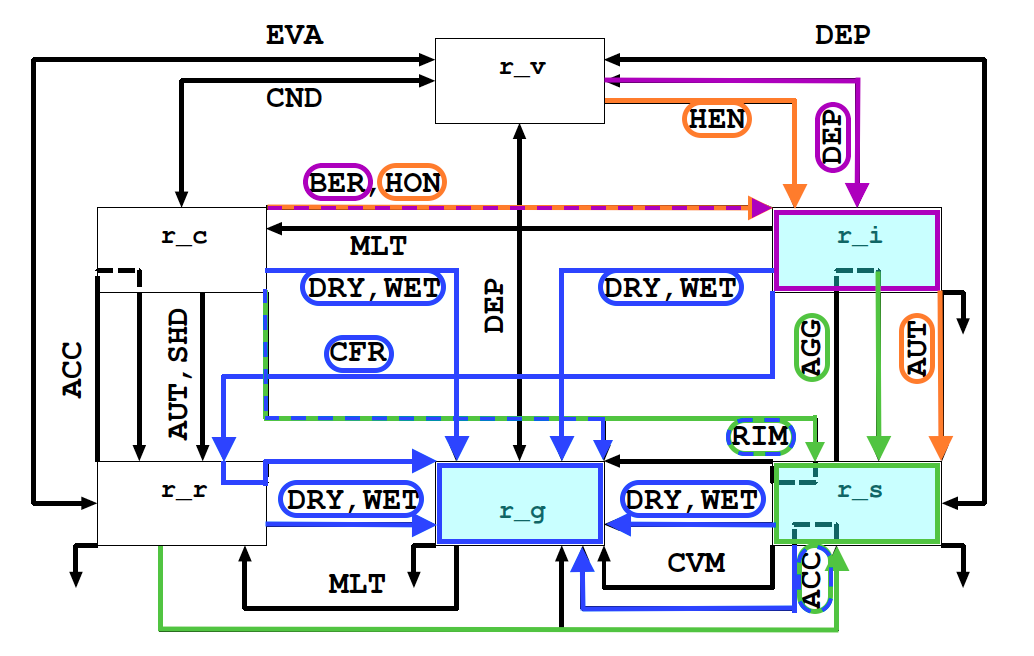
\includegraphics[width=\textwidth]{./fig_MEPS/ICE3_scheme_copy}
	%	\end{subfigure}
	\caption{Microphysical processes for mixed phase clouds in the ICE3 scheme adapted from \cite{meteo_france_meso-nh_2009}. In orange the initiation processes for primary ice r$_i$ and snowflakes r$_s$. The growing processes of r$_i$ is shown in purple and for r$_s$ in green. Graupel particles, r$_g$, grow from existent particles and the processes are shown in blue. }\label{fig:ICE3_scheme}
\end{figure}
%%%%%%%%%%%%%%%%%%%%%%%%%%%%%%%%%%%%%%%%%%%%%%%%%%%%%%%%%%%%%%%%%%%%%%%%%%
\newline
\cite{meteo_france_meso-nh_2009} documentation suggests starting the microphysics in the ICE3 scheme with 'slow' processes such as homogeneous and heterogeneous nucleation (HON, HEN), vapour deposition of snow and graupel particles (DEP), aggregation (AGG) and auto conversion (AUT), for ice processes right side in \Cref{fig:ICE3_scheme}. The second step is to initiate the warm processes left side in \Cref{fig:ICE3_scheme}. Then include the aggregation and conversion-melting (CVM) for snowflakes and contact freezing of raindrops (CFR). Add AGG and melting for graupel (MLT), and then the melting from pristine ice  and the Wegener-Bergeron-Findeisen (BER) effect and lastly the sedimentation terms.  \\
\Cref{fig:ICE3_scheme} shows the summary of the microphysical processes for mixed phase clouds. The study focuses mostly on solid precipitation particles and therefore only the initiation and growth of pristine ice crystals r$_i$, snowflakes r$_s$, and rimed crystals r$_g$ is presented. 
\\
Following \cite{pinty_mixed-phased_1998} and \Cref{fig:ICE3_scheme} it can be seen how AROME performs the ice production. Orange lines in \Cref{fig:ICE3_scheme} show the initiation of pristine ice crystals and snowflakes. In purple the growth mechanisms of r$_i$ (BER,DEP). Green lines demonstrate the expansion of the snowflakes (RIM, AGG, ACC). Graupel (r$_g$) forms as an effect of heavy riming (RIM), by collision of larger raindrops with snowflakes (ACC), by WET/DRY growth or by contact freezing of raindrops (CFR). All graupel growth processes are indicated by blue lines in \Cref{fig:ICE3_scheme}, were hail formation is included. 

% are the primary ice crystals activated by either heterogeneous nucleation (HEN), when some ice nuclei are present or by homogeneous nucleation (HON), when the atmospheric temperature is below \SI{-35}{\celsius}. The growing process for these particles can be the Bergeron-Findeisen process (BER) or deposition of water vapour (DEP). \\
% Snow particles are initiated by auto conversion (AUT) of r$_i$ and grow by the riming of cloud droplets (RIM) or rain droplets (ACC), and by collection of small pristine crystals (AGG), indicated by the green lines in \Cref{fig:ICE3_scheme}. \\
% As indicated by the blue lines in \Cref{fig:ICE3_scheme} are graupel an effect of heavy riming and grow in the scheme if the riming aggregates are of larger diameter size than \SI{7}{\mm} \citep{meteo_france_meso-nh_2009}. As indicated can graupel also grow when larger colliding raindrops reshape snowflakes to graupel (ACC). Furthermore, is graupel growth affected by wet or dry (WET, DRY) accretion, when the surface temperature of graupel is larger than the environmental temperature. DRY graupel expansion happens as long as the surface temperature is less that the surrounding temperature, then collected drops will freeze. WET graupel growth appears, when a liquid film is on the surface of the graupel particle (surface temperature larger than surrounding) then the liquid condensate is shed away, and hail will be formed. In ICE3 is hail not specifically included it is mixed in to the graupel category and therefore a distinction between the two categories cannot be made. 

%
\subsection{Adjustment of ICE3 inside MEPS}
% refinement for AROME 
Since the ICE3 scheme showed some weaknesses for the winter month, \cite{muller_arome-metcoop:_2017} introduced some modifications. 
During cold conditions the ICE3-scheme showed too low temperature at two meter, too much ice fog and all year long was the occurrence of cirrus overestimated. After implementing the modifications described in \cite{muller_arome-metcoop:_2017} the two meter temperature bias was reduced as well as an improvement of low-level clouds was shown. A negative aspect of these adjustments was that the occurrence of fog increased.%, by an error in the surface scheme.

% %%%%%%%%%%%%%%%%%%%%%%%%%%%%%%%%%%%%%%%%%%%%%%%%%%%%%%%%%%%%%%%%%%%%%%%%%%
% %%%%%%%%%%%%%%%%%%%%%%%%%%%%%%%%%%%%%%%%%%%%%%%%%%%%%%%%%%%%%%%%%%%%%%%%%%
% %%%%%%%%% SURFEX %%%%%%%%%%%%%%
% \section{SURFEX}
% \cite{masson_surfexv7.2_2013} \\
% SURFEX stands for 'surface externalisée' and is introduced into NWP models to ensure the consistent treatment of surface processes. It simulates the exchange of energy between four surface types and the atmosphere \citep{homleid_verification_2016}.

%%%%%%%%%%%%%%%%%%%%%%%%%%%%%%%%%%%%%%%%%%%%%%%%%%%%%%%%%%%%%%%%%%%%%%%%%%
%%%%%%%%%%%%%%%%%%%%%%%%%%%%%%%%%%%%%%%%%%%%%%%%%%%%%%%%%%%%%%%%%%%%%%%%%%














%%%%%%%%%%%%%%%%%%%%%%%%%%%%%%%%%%%%%%%%%%%%%%%%%%%%%%%%%%%%%%%%%%%%%%%%%%
%%%%%%%%%%%%%%%%%%%%%%%%%%%%%%%%%%%%%%%%%%%%%%%%%%%%%%%%%%%%%%%%%%%%%%%%%%
% %%% ***************** CHAPTER DATA PROCESSING ***************** %%%
% !TeX spellcheck = en_GB
\section{Computing Snowfall Quantities} \label{sec:data_proc}
%The previous \Cref{sec:retrieval,sec:MEPS} represented the details on retrieving snowfall amounts from the optimal estimation retrieval and the forecast model outputs. 
The following section will describe how the different variables where processed to achieve a comparison between the retrieved values and the forecast model output. 

%%%%%%%%%%%%%%%%%%%%%%%%%%%%%%%%%%%%%%%%%%%%%%%%%%%%%%%%%%%%%%%%%%%%%%%%%%
%%%%%%%%% THICKNESS IN MEPS %%%%%%%%%%%%%%
\subsection{Layer Thickness in MEPS}\label{sec:layer_thickness}
To compare the measurements from the surface with the MEPS data, the closest grid point to Haukeliseter, is used. The closest grid point to Haukeliseter is \ang{59.80}\,N, \ang{7.22}\,E.
\\
MEPS has a vertical resolution in hybrid sigma pressure coordinates, were one is at the surface and decreases with height. To calculate the actual vertical pressure in \SI{}{\Pa}, a formula is provided in the OPeNDAP Dataset of \texttt{meps\_full\_2\_5km\_*.nc} by the \citet{norwegian_meteorological_institute_met_2016}.  
\begin{align}
	p(n,k,j,i) = a_p(k) + b(k) \cdot p_s(n,j,i) \qquad [\SI{}{\Pa}].
	\label{eq:hybrid_sigma_pressure}
\end{align}
$p_s$ is the surface air pressure in \SI{}{\Pa}, and information about the variables $a_p$, $b$ are not given from the access form. \textcolor{red}{Find reference for sigma-hybrid coordinate transformation equation.}  
\\
The next step was to convert pressure-levels into actual heights by the use of the hypsometric equation. Here, the air temperature in model levels is used to calculate the mean temperature of each layer. 
\begin{align}
	\overline{T} = \dfrac{\int\limits_{p2}^{p1} T \partial ln p}{\int\limits_{p2}^{p1}\partial ln p} \qquad [\SI{}{\kelvin}]
	\label{eq:T_avg}
\end{align}
For the numerical integration, the Simpson rule was used, which is a build-in function in Python. \\
\citet{martin_mid-latitude_2006} presents steps of differentiating the hypsometric equation by using the virtual air temperature. But when the atmospheric mixing ratio is large, will the virtual temperature only be \SI{1}{\percent} larger than the actual air temperature. Since the error is little calculations are done with the provided air temperature in model levels.
\\
The thickness, $\Delta z$, of each layer is then be found by using the hypsometric equation from \citet{martin_mid-latitude_2006} and the previously calculated mean temperature (\Cref{eq:T_avg}):
\begin{equation}
\begin{split}
\Delta z  = z_2 - z_1 
& = \frac{R_d \overline{T}}{g} ln\left(\frac{p_1}{p_2} \right) \qquad [\SI{}{\metre}]
\end{split}
\label{eq:hypsometric}
\end{equation}
where $R_d$ is gas constant for dry air with a value of \SI{287}{\joule\per\kilogram\per\kelvin},  standard gravity $g\,=\,$\SI{9.81}{\metre\per\square\second}. $p_1$ and $p_2$ are the pressure levels at lower and higher levels, respectively ($p_2 < p_1$).
To gain the respective height of each pressure layer, $\Delta z$ is summed.

%%%%%%%%%%%%%%%%%%%%%%%%%%%%%%%%%%%%%%%%%%%%%%%%%%%%%%%%%%%%%%%%%%%%%%%%%%
%%%%%%%%% SWC %%%%%%%%%%%%%%
\subsection{Snow Water Content}
To get a valid comparison between the SWC from the optimal estimation retrieval and the results from MEPS, the SWC is averaged over each hour. Taking the model initialisation of MEPS at \SI{0}{\UTC} the model produces forecast values at \SI{0}{}, \SI{1}{}, \SI{2}{}, $\ldots$, \SI{22}{}, \SI{23}{}, $\ldots$, \SI{66}{\UTC}. To approach hourly mean values from the retrieval SWC an average over \SI{30}{\minute} prior and \SI{29}{\minute} after each full hour is performed. This leads to a match of the average value at the same time as from MEPS. \\
Since MEPS has a higher vertical resolution than the optimal estimation snowfall retrieval each vertical profile of SWC is averaged every \SI{200}{\metre}. To accomplish the same vertical resolution only values above \SI{100}{\metre} are used to start at the same range height as given from the MRR (\Cref{sec:MRR}).
\\
Within the output from MEPS snow water content does not exist for each model layer. Hence the calculation of the SWC is performed by using the three solid precipitation categories given in MEPS. Namely the instantaneous mixing ratio of snowfall ($r_s$), graupel fall ($r_g$) and the atmosphere cloud ice content ($r_i$). The mixing ratios are represented in \SI{}{\kg\per\kg} and a transformation to \SI{}{\g\per\cubic\meter} is performed. Densities in each model level ($\rho_{ml}$) are calculated and then multiplied with the sum of the solid precipitation mixing ratio. 
\begin{align}
	\rho_{ml} & = \frac{p_{ml}}{R_d T} & \quad [\SI{}{\kg\per\cubic\meter}]  \\
	SWC_{ml} & = \rho_{ml} \cdot (r_s + r_g + r_i)_{ml} \cdot \num{e6} & \quad [\SI{}{\g\per\cubic\meter}].
	\label{eq:SWC_ml}
\end{align}

%%%%%%%%%%%%%%%%%%%%%%%%%%%%%%%%%%%%%%%%%%%%%%%%%%%%%%%%%%%%%%%%%%%%%%%%%%
%%%%%%%%% SWP %%%%%%%%%%%%%%
\subsection{Snow Water Path}\label{sec:SWP}
The snow water path (SWP) is the vertically integrated value of the averaged SWC (\Cref{eq:SWC,eq:SWC_ml}), where the numerical Simpson's integration is applied.  
\begin{equation}
\begin{split}
\int_{h_0}^{h_1=\SI{3000}{\metre}} \text{SWC}(h) \, dh \approx 
\frac{h_1 - h_0}{6}  & \left[ \text{SWC}(h_0)    + \text{SWC}(h_1)   \vphantom{\frac{h_0 + h1}{2}} \right. \\ 
& \left. + 4 \text{SWC}\left(\frac{h_0 + h1}{2}\right)  
\right] \qquad [\SI{}{\g\per\square\meter}]
\end{split}
\label{eq:SWP}
\end{equation}
The snow water path is a measure of the weight of ice particles per unit area. It indicates the total amount of ice in the atmosphere.
%%%%%%%%%%%%%%%%%%%%%%%%%%%%%%%%%%%%%%%%%%%%%%%%%%%%%%%%%%%%%%%%%%%%%%%%%%
\section{Statistical Methods for Analysing Data}
\textcolor{red}{Something to get a flow}
%%%%%%%%% Ensemble spread %%%%%%%%%%%%%%
\subsection{Ensemble Mean and Coefficient of Variation}\label{sec:ens_mean_spread}
\textcolor{red}{Check literature of meaning} \\
The ensemble mean is the average of all ten ensemble members of MEPS.
\begin{align}
	\bar{x} & = \frac{\sum_{i=1}^n x_i}{N} \label{eq:meanMEPS}
\end{align}
which is the standard deviation of the ten ensemble members divided by the mean of all ensemble members. This coefficient gives the possibility to compare the SWC results for different days with different values. 
%It follows for even a low ensemble spread of SWC (standard deviation of all ensemble members) then the different members do not need to be less variable.
The coefficient of variation shows the variation around the center or control run.
The standard deviation is defined as:
\begin{align}
	\sigma & = \sqrt{\frac{\sum_{i=1}^n (x_i - \bar{x})^2}{N-1}} \label{eq:stdMEPS}
\end{align}
which follows for the coefficient of variation:
\begin{align}
	CV & = \frac{\sigma}{\bar{x}}
\end{align}
% \\
% To verify how well MEPS performed during the Christmas storm a variation of the SWC is calculated. For this, the standard deviation (\Cref{eq:stdMEPS}) is divided by the ensemble mean (\Cref{eq:meanMEPS}).

%%%%%%%%%%%%%%%%%%%%%%%%%%%%%%%%%%%%%%%%%%%%%%%%%%%%%%%%%%%%%%%%%%%%%%%%%%
%%%%%%%%% MAE & ME %%%%%%%%%%%%%%
\subsection{Mean Error and Mean Absolute Error}
The mean error for the each ensemble member is calculated with: 
\begin{align}
	ME = \frac{\sum_{i=1}^n MEPS_{ens} - DoFe_{obs}}{N}
\end{align}
where $MEPS_{ens}$ represents the value of each ensemble member and $DoFe_{obs}$ defines the observation from the double fence. For the mean absolute error follows then:
\begin{align}
	MAE = \frac{\sum_{i=1}^n \left| MEPS_{ens} - DoFe_{obs}\right|}{N} \label{eq:MAE}
\end{align}

%%%%%%%%%%%%%%%%%%%%%%%%%%%%%%%%%%%%%%%%%%%%%%%%%%%%%%%%%%%%%%%%%%%%%%%%%%
%%%%%%%%% %Diff, %Avg Diff %%%%%%%%%%%%%%
\subsection{Percent Difference and Average Difference}
The percentage difference presented in the results (\Cref{tab:res:ret_error} and \textcolor{red}{add for MEPS}) are calculated by:
\begin{align}
	\SI{}{\percent} \text{Difference} & = \frac{SF - DoFe_{obs}}{DoFe_{obs}} \times 100
\end{align}
$SF$ presents the snowfall from the retrieval or the MEPS ensemble forecast. The average is then taken from all \SI{}{\percent} Difference values to see the difference of the Christmas storm 2016.


%%%%%%%%%%%%%%%%%%%%%%%%%%%%%%%%%%%%%%%%%%%%%%%%%%%%%%%%%%%%%%%%%%%%%%%%%%